\documentclass[11pt]{article}
\usepackage{amsmath, amsthm, amssymb, pdfpages} 
\usepackage{fullpage}
\usepackage{hyperref}
\usepackage{graphicx}
\usepackage[capitalize]{cleveref}
\usepackage[CaptionBefore]{fltpage} % for large figures, captions go on prev page

% options for pretty tables from CSV files
\usepackage{booktabs,csvsimple,siunitx}
% for commas in big numbers (i.e. "3,000,000")
\sisetup{group-separator={,}}

% next three for UTF8 to work (for non-ASCII names to work without awkward codes)
\usepackage[T1]{fontenc}
\usepackage{textcomp}
\usepackage[utf8]{inputenc}

% import biblatex with prefered settings
% loads biblatex with all the nice standard options that John determined some time ago!
% this version uses a ``Harvard'' style (first author last name, year in parentheses).
% also loads xpatch

% biblatex
% harvard style
\usepackage[style=authoryear,natbib,maxcitenames=2,doi=false,isbn=false,url=false,backend=bibtex]{biblatex}
% numeric style
%% \usepackage[style=numeric-comp,sorting=none,giveninits=true,
%%                      doi=false,isbn=false,url=false,backend=bibtex]{biblatex}
% remove "In: " before journal title
\renewbibmacro{in:}{}
% remove language
\AtEveryBibitem{\clearlist{language}}
% remove month
\AtEveryBibitem{\clearfield{month}}
% and also notes
\AtEveryBibitem{\clearfield{note}}
% remove dots between volume and issue
\usepackage{xpatch}
\xpatchbibmacro{volume+number+eid}{%
  \setunit*{\adddot}%
}{%
}{}{}
% put issue in parentheses
\DeclareFieldFormat[article]{number}{\mkbibparens{#1}}


\bibliography{zotero, dummy}

% path of images
\graphicspath{ {../data/} }

% define shortcuts for awkward math symbols
% this also helps us change them more easily later, if needed
\newcommand{\rmsd}{\text{SRMSD}_p}
\newcommand{\auc}{\text{AUC}_\text{PR}}

\usepackage{kinshipsymbols}

% double line spacing (PLoS wants this)
\usepackage{setspace}
\doublespacing
% original, smaller spacing
%\renewcommand{\baselinestretch}{1.2}

% cool automatic supplemental figures/tables!
% http://bytesizebio.net/2013/03/11/adding-supplementary-tables-and-figures-in-latex/
% with some additions
\newcommand{\beginsupplement}{%
  \setcounter{table}{0}
  \renewcommand{\thetable}{S\arabic{table}}%
  \setcounter{figure}{0}
  \renewcommand{\thefigure}{S\arabic{figure}}%
  \setcounter{section}{0}
  \renewcommand{\thesection}{S\arabic{section}}%
  \setcounter{equation}{0}
  \renewcommand{\theequation}{S\arabic{equation}}%
  \setcounter{page}{1}
  \renewcommand{\thepage}{S\arabic{page}}%
}


% OLD: Testing the effectiveness of principal components in adjusting for relatedness in genetic association studies
\title{\Large \textbf{
    Limitations of principal components in quantitative genetic association models for human studies
  }}
\author{Yiqi Yao$^1$, Alejandro Ochoa$^{1,2,*}$}
\date{}

\begin{document}
\maketitle

\noindent
$^1$ Department of Biostatistics and Bioinformatics, Duke University, Durham, NC 27705, USA \\
$^2$ Duke Center for Statistical Genetics and Genomics, Duke University, Durham, NC 27705, USA \\
$^*$ Corresponding author: \texttt{alejandro.ochoa@duke.edu}

\begin{abstract}
  Principal Component Analysis (PCA) and the Linear Mixed-Effects Model (LMM), sometimes in combination, are the most common modern models for genetic association.
  Previous PCA-LMM comparisons give mixed results and unclear guidance, and have several limitations, including not varying the number of principal components (PCs), simulating overly simple population structures, and inconsistent use of real data and power evaluations.
  In this work, we thoroughly evaluate PCA and LMM both with varying number of PCs in new realistic genotype and complex trait simulations including admixed families, trees, and large real multiethnic human genotype datasets (1000 Genomes Project, the Human Genome Diversity Panel, and Human Origins) with simulated traits.
  We find that LMM without PCs performs best in all cases, with the largest effects in the family simulation and all real human datasets.
  We determined that the large gaps in PCA to LMM performance on the real human datasets is due to the high-dimensional family structure stemming from large numbers of distant relatives, and not from the smaller number of highly related pairs.
  While it was known that PCA fails on family data, here we report a strong effect on association of cryptic family relatedness in several genetically diverse human datasets, a problem that is not avoided with the common practice of pruning high-relatedness individual pairs.
  Overall, this work better characterizes the severe limitations of PCA compared to LMM in modeling the complex relatedness structures present in real multiethnic human data and its impact in association studies.
\end{abstract}

% used for ASHG abstract
% \textbf{Keywords:} genetic association, statistical genetics, population structure, complex traits, genetic diversity.

\textbf{Abbreviations:}
PCA: principal component analysis;
PCs: principal components;
LMM: linear mixed-effects model;
FES: fixed effect sizes;
RC: random coefficients;
WGS: whole genome sequencing.

\section{Introduction} 

% need for specialized approaches
The goal of a genetic association study is to identify loci whose genotype variation is significantly correlated to given trait.
An important, implicit assumption by naive association tests is that, under the null hypothesis, genotypes are unstructured: drawn independently from a common allele frequency.
This assumption does not hold for structured populations, which includes multiethnic cohorts and admixed individuals, and for family data.
When naive or insufficient approaches are applied to structured populations or family data, association statistics become miscalibrated relative to the null expectation, resulting in greater numbers of false positives than expected and loss of power \citep{devlin_genomic_1999, voight_confounding_2005, astle_population_2009}.
Therefore, many specialized approaches have been developed for genetic association in structured data.
Here we focus on extensively evaluating the two most popular association models: PCA and LMM.

% PCA
Genetic association with PCA consists of including the top eigenvectors of the population kinship matrix as covariates in a generalized linear model \citep{zhang_semiparametric_2003, price_principal_2006, bouaziz_accounting_2011}.
These top eigenvectors are commonly referred to as PCs in genetics \citep{patterson_population_2006}, the convention adopted here, but it is worth noting that in other fields PCs instead denote the projections of loci onto eigenvectors \citep{jolliffe_principal_2002}.
The direct ancestor of PCA association is structured association, in which inferred ancestry or admixture proportions are used as regression covariates \citep{pritchard_association_2000}.
These models are deeply connected because PCs map to ancestry empirically (\textit{e.g.}, \cite{alexander_fast_2009, zhou_strong_2016}) and theoretically \citep{mcvean_genealogical_2009,zheng_eigenanalysis_2016,cabreros_likelihood-free_2019}, and they work as well as global ancestry in association studies but are estimated more easily \citep{patterson_population_2006, zhao_arabidopsis_2007, alexander_fast_2009, bouaziz_accounting_2011}.
The strength of PCA is its simplicity, which as covariates can be readily integrated into more complex models, such as haplotype association \citep{xu_detecting_2014} and polygenic models \citep{qian_fast_2020}.
However, PCA fundamentally assumes that relatedness is low-dimensional, which may limit its applicability.
PCA is known to be inadequate for data containing family structure \citep{patterson_population_2006, thornton_roadtrips:_2010, price_new_2010}, which is called ``cryptic relatedness'' when it is unknown to the researchers, but no other specific troublesome scenarios have been confidently identified.
Recent work has focused on developing more scalable versions of the PCA algorithm \citep{lee_sparse_2012, abraham_fast_2014, galinsky_fast_2016, abraham_flashpca2:_2017, agrawal_scalable_2020}.
PCA remains a popular and powerful approach for association studies.

% LMM
The other dominant association model for structured populations is the LMM, in which this structure is a random effect drawn from a multivariate Normal model parametrized by the kinship matrix.
Unlike PCA, LMM does not assume that relatedness is low-dimensional, and explicitly models family structure via the kinship matrix.
Early LMMs required kinship matrices estimated from known pedigrees or which otherwise captured family-level relatedness only \citep{yu_unified_2006, zhao_arabidopsis_2007}.
Modern LMMs estimate kinship from genotypes using a non-parametric estimator, often referred to as a genetic relationship matrix, that captures the combined covariance due to recent family relatedness and ancestral population structure \citep{kang_efficient_2008, astle_population_2009, ochoa_estimating_2021}.
The classic LMM assumes a quantitative (continuous) complex trait, the focus of our work.
Although case-control (binary) traits and their underlying ascertainment are theoretically a challenge \citep{yang_advantages_2014}, LMMs have been applied successfully to balanced case-control studies \citep{astle_population_2009, kang_variance_2010} and simulations \citep{price_new_2010, wu_comparison_2011, sul_mixed_2013}, and have been adapted for unbalanced case-control studies \citep{zhou_efficiently_2018}.
However, LMMs tend to be considerably slower than PCA and other models, so much effort has been devoted to improving their runtime and scalability \citep{aulchenko_genomewide_2007, kang_efficient_2008, kang_variance_2010, zhang_mixed_2010, lippert_fast_2011, yang_gcta:_2011, listgarten_improved_2012, zhou_genome-wide_2012, svishcheva_rapid_2012, loh_efficient_2015, zhou_efficiently_2018}.

% LMM+PCA
An LMM variant that incorporates PCs as fixed covariates is tested thoroughly in our work.
Since PCs are the top eigenvectors of the same kinship matrix estimate used in modern LMMs \citep{astle_population_2009, hoffman_correcting_2013}, then population structure is modeled twice in an LMM with PCs.
However, some previous work has found the apparent redundancy of an LMM with PCs beneficial \citep{price_new_2010, tucker_improving_2014}, while others did not \citep{liu_controlling_2011}, and the approach continues to be used \citep{zeng_signatures_2018}.
It is worth noting that early LMMs had a different arrangement, as their kinship matrices captured family relatedness only, so population structure had to be modeled separately, in practice as admixture fractions instead of PCs \citep{yu_unified_2006, zhao_arabidopsis_2007}.

\begin{table}[b!]
  \centering
  \small
  \caption{
    \textbf{Previous PCA-LMM evaluations in the literature.}
  }
  \label{tab:lit}
  \begin{tabular}{l|ccc|ccccc}
    \toprule
                & \multicolumn{3}{c|}{Sim. Genotypes} & \\
    Publication & Type\textsuperscript{a} & $K$\textsuperscript{b} & \Fst\textsuperscript{c} & Real\textsuperscript{d} & Trait\textsuperscript{e} & Power & PCs ($r$) & Best \\
    \midrule
    % Publication                & Sim &    K &     Fst &       Re & Ph &      Pow & PCAr & Best\\
    \cite{zhao_arabidopsis_2007} &     &      &         &\checkmark&  Q &\checkmark&    8 & LMM \\
    \cite{astle_population_2009} &   I &    3 &    0.10 &          & CC &\checkmark&   10 & Tie \\
    \cite{kang_variance_2010}    &     &      &         &\checkmark&Both&          &2-100 & LMM \\
    \cite{price_new_2010}        &I, F &    2 &    0.01 &          & CC &          &    1 & Mixed \\
    \cite{wu_comparison_2011}    &I, A &  2-4 &    0.01 &          & CC &\checkmark&   10 & Mixed \\
    \cite{liu_controlling_2011}  &S, A &  2-3 &       R &          &  Q &\checkmark&   10 & Tie \\
    \cite{sul_mixed_2013}        &   I &    2 &    0.01 &          & CC &          &    1 & Tie \\
    \cite{tucker_improving_2014} &   I &    2 &    0.05 &\checkmark&Both&\checkmark&    5 & Tie \\
    \cite{yang_advantages_2014}  &     &      &         &\checkmark& CC &\checkmark&    5 & Tie \\
    \cite{song_testing_2015}     &S, A &  2-3 &       R &          &  Q &          &    3 & LMM \\
    \cite{loh_efficient_2015}    &     &      &         &\checkmark&  Q &\checkmark&   10 & LMM \\
    \cite{liu_iterative_2016}    &     &      &         &\checkmark&  Q &\checkmark&  3-6 & LMM \\ 
    \cite{sul_population_2018}   &     &      &         &\checkmark&  Q &          &  100 & LMM \\
    This work                    &A, T, F&10-243&$\le$0.25&\checkmark&  Q &\checkmark& 0-90 & LMM \\
    \bottomrule
  \end{tabular}
  \begin{flushleft} 
    \textsuperscript{a}Genotype simulation types. I: Independent subpopulations; S: subpopulations (with parameters drawn from real data); A: Admixture; T: Tree; F: Family.\\
    \textsuperscript{b}Model dimensionality (number of subpopulations or ancestries)\\
    \textsuperscript{c}R: simulated parameters based on real data, \Fst not reported.\\
    \textsuperscript{d}Evaluations using unmodified real genotypes.\\
    \textsuperscript{e}Q: quantitative; CC: case-control.
  \end{flushleft}
\end{table}


% LMM and PCA are similar
LMM and PCA are closely related models \citep{astle_population_2009, hoffman_correcting_2013}, which suggests similar performance in some cases, particularly low-dimensional relatedness.
Direct comparisons have yielded mixed results, with several studies finding superior performance for LMM (notably from papers promoting advances in LMMs) while many others report comparable performance (\cref{tab:lit}).
None of these papers find that PCA outperforms LMM decisively, although PCA occasionally performs better in isolated and artificial cases or individual measures (often with unknown significance).
Several patterns emerged in our literature search, which may explain these discrepancies.
Previous studies were generally divided into two types: those that employed exclusively simulated genotypes, versus exclusively real genotypes (only one study used both).
We find that the simulated genotype studies, which tended to have low dimensionalities and differentiation (\Fst), were more likely to report ties or mixed results (6/7), whereas real genotypes tended to clearly favor LMMs (5/7).
Similarly, 6/8 papers that use quantitative traits favor LMMs, whereas 5/7 papers that used case-control traits gave ties or mixed results (the only factor we do not explore).
Other limitations of previous evaluations are that, although all measured type I error (or proxies such as inflation factors or QQ plots), a large fraction (5/13) did not measure power (including proxies such as ROC curves), and only two reported trying more than one number of PCs when evaluating PCA.
Lastly, no consensus has emerged as to why LMM might outperform PCA or vice versa \citep{price_new_2010, sul_mixed_2013, price_response_2013, hoffman_correcting_2013}, or which features of the real datasets are critical for the LMM advantage, with the exception that LMM handles family relatedness whereas PCA does not, leaving users confused as to when it is appropriate to use PCA.
To better evaluate PCA and LMM, our work includes more complex, high-dimensional genotype simulations with differentiation matching that of multiethnic human cohorts, as well as real genotypes, we vary the number of PCs, and consistently measure robust proxies for type I error and power.

% this work
In this work, we study the performance of the PCA and LMM association models, characterizing their behavior under various numbers of PCs (included in LMM too).
We use genotype simulations (admixture, family, and tree models) and three real datasets: the 1000 Genomes Project \citep{the_1000_genomes_project_consortium_map_2010, 1000_genomes_project_consortium_integrated_2012}, the Human Genome Diversity Panel (HGDP) \citep{cann_human_2002, rosenberg_genetic_2002, bergstrom_insights_2020}, and Human Origins \citep{patterson_ancient_2012, lazaridis_ancient_2014, lazaridis_genomic_2016, skoglund_genomic_2016}.
We simulate quantitative traits from two models: fixed effect sizes (FES; coefficients inverse to allele frequency) that matches real data \citep{park_distribution_2011, zeng_signatures_2018, oconnor_extreme_2019} and corresponds to high pleiotropy and strong balancing selection \citep{simons_population_2018} and strong negative selection \citep{zeng_signatures_2018, oconnor_extreme_2019}, which are appropriate assumptions for diseases; and random coefficients (RC; independent of allele frequency) that corresponds to neutral traits \citep{zeng_signatures_2018, simons_population_2018}.
Across all tests, LMM without PCs consistently performs best, and greatly outperforms PCA in the family simulation and in all real datasets.
The tree simulations do not recapitulate the real data results, suggesting that family-like structure in real data is the reason for poor PCA performance.
Lastly, removing up to 4th degree relatives in the real datasets recapitulates poor PCA performance, showing that the more numerous distant relatives explain the result.
All together, we find that LMMs without PCs are generally a preferable association model, and present novel simulation and evaluation approaches to measure the performance of these and other genetic association approaches.

\section{Results}

The success of our investigation hinges on simulating a variety of population structures and quantitative trait models, introduced first, which have the goal of capturing all the essential features present in genetically diverse human studies, and compared directly to evaluations based on real genotypes.
Then we summarize the evaluation methods and present the results.

\subsection{Overview of genotype simulations and real datasets}

We utilized three real genotype datasets and simulated genotypes from six population structure scenarios to cover various features of interest (\cref{tab:human_sum}).
We will introduce them here in sets of three, as they appear in the rest of our results.
The population structures are also conveniently visualized in \cref{fig:kinship} using \texttt{popkin} to estimate population kinship matrices (which combine family and population relatedness) without bias \citep{ochoa_estimating_2021}.

\begin{table}[hb!]
  \centering
  \footnotesize
  \caption{
    \textbf{Features of simulated and real human genotype datasets.}
  }
  \label{tab:human_sum}
  % read and automatically format data from a TSV file!
  \sisetup{ table-format = 2, table-number-alignment = right }
  \csvreader[
  tabular = {llSSrSS[table-number-alignment=left]},
  separator = tab,
  table head = \toprule Dataset & Type & {Loci ($m$)} & {Ind.~($n$)} & {Subpops.\textsuperscript{a}~($K$)} & {Causal loci\textsuperscript{b} ($m_1$)} & \Fst\textsuperscript{c} \\\midrule,
  late after last line = \\\bottomrule
  ]{../data/dimensions.txt}{}{\csvlinetotablerow}
  \begin{flushleft} 
    \textsuperscript{a}For admixed family, ignores dimensionality of 20 generation pedigree structure.
    For real datasets, lower range is continental subpopulations, upper range is number of fine-grained subpopulations.\\
    \textsuperscript{b}$m_1 = n / 10$ in all cases to balance power across dataset.\\
    \textsuperscript{c}Model parameter for simulations, estimated value on real datasets.
  \end{flushleft}
\end{table}

\begin{FPfigure}%[H]
  \centering
  \includegraphics[width=\textwidth,height=\textheight,keepaspectratio]{kinship.pdf}
  \caption{
    {\bf Population structures of simulated and real human genotype datasets.}
    First two columns are population kinship matrices as heatmaps: 
    Individuals are placed along both x- and y-axes, kinship represented with color (lighter is closer to zero, darker red are higher values).
    Diagonal shows inbreeding values.
    \textbf{A.}
    Admixture scenario for both Large and Small simulations.
    \textbf{B.}
    Last generation of 20-generation admixed family, shows larger kinship values near diagonal corresponding to siblings, first cousins, etc.
    \textbf{C.}
    Minor allele frequency (MAF) distributions.
    Real datasets and tree simulations had $\text{MAF} \ge 0.01$ filter.
    \textbf{D.}
    Human Origins is an array dataset from a large diversity of humans from around the world.
    \textbf{G.}
    Human Genome Diversity Panel (HGDP) is a WGS dataset from native populations around the world.
    \textbf{J.}
    1000 Genomes Project is a WGS dataset sampling cosmopolitan populations around the world.
    \textbf{F,I,L.}
    Trees between subpopulations fit to real data, used to draw genotypes in simulations.
    \textbf{E,H,K.}
    Simulations from trees fit to the real data recapitulate structure at the subpopulation level.
  }
  \label{fig:kinship}
\end{FPfigure}


% SIM
The first set of three simulated genotypes are based on an admixture model from 10 subpopulations (\cref{fig:kinship}A) \citep{ochoa_estimating_2021, gopalan_scaling_2016, cabreros_likelihood-free_2019}.
The ``large'' version has 1000 individuals and illustrates asymptotic performance, while the ``small'' simulation has 100 individuals to illustrate model overfitting.
The ``family'' simulation has admixed founders and draws a 20-generation random pedigree with assortative mating, resulting in a complex joint family and ancestry structure in the last generation (\cref{fig:kinship}B).

% REAL
The second set of three are the real human datasets: Human Origins (\cref{fig:kinship}D), HGDP (\cref{fig:kinship}G), and 1000 Genomes (\cref{fig:kinship}J).
All of these represent global human diversity with varying resolutions, making them of great interest as representatives of proposed multiethnic studies.
These datasets had loci filtered to avoid linkage disequilibrium, to simplify our evaluation, and are enriched for small minor allele frequencies, even after excluding rare variants (MAF < 1\%; \cref{fig:kinship}C).

% REAL-SIM
Last are tree simulations (\cref{fig:kinship}F,I,L), fit to the kinship of each real human dataset (\cref{fig:kinship}E,H,K), and used to draw genotypes.
Ancestral allele frequencies were constructed to mimic the real allele frequency skews (\cref{fig:kinship}C).
By design, these tree simulations do not contain any family structure.

\subsection{Overview of trait simulation models}

All traits in this work are simulated, starting from (real or simulated) genotypes and picking causal loci randomly.
We repeated all of our tests for two additive quantitative trait models, \textit{fixed effect sizes} (FES) and \textit{random coefficients} (RC), which differ in how causal coefficients are constructed.
In both cases coefficients are scaled to yield a heritability of 0.8.

The FES simulation selects coefficients $\beta_i$ such that the effect size $2 \beta_i^2 \pit ( 1 - \pit )$ have the same value at every locus $i$, where \pit is the ancestral allele frequency of the simulation ($T$ is the ancestral population).
Our simple model captures the rough inverse relationship between coefficient and minor allele frequency that arises under strong negative and balancing selection and has been observed in numerous diseases and other traits \citep{park_distribution_2011, zeng_signatures_2018, simons_population_2018, oconnor_extreme_2019}, and thus the focus of our results.

The RC simulation selects coefficients randomly, independent of allele frequency, which corresponds to neutral traits \citep{zeng_signatures_2018, simons_population_2018}.
The resulting effect size distributions are wider, which reduces association power and effective polygenicity compared to FES.

\subsection{Overview of evaluations}

% MEASURES
Since our quantitative traits are simulated, true causal loci are known, resulting in known true positives, false positives, and false negatives.
We employ two complementary measures:
(1) $\rmsd$ (p-value signed root mean square deviation) measures null p-value uniformity (closer to zero is better), and
(2) $\auc$ (precision-recall area under the curve) measures causal locus classification performance (higher is better; \cref{fig:measures_illustration}).
$\rmsd$ is a more robust alternative to the common inflation factor $\lambda$ and type I error measures; we found a good correspondence between $\lambda$ and $\rmsd$, and determined that the threshold $\rmsd > 0.01$ corresponds to $\lambda > 1.06$ (\cref{fig:rmsd_lambda}) and thus evidence of miscalibration close to the rule of thumb of $\lambda > 1.05$ \citep{price_new_2010}.
$\auc$ has been used to evaluate association models \citep{rakitsch_lasso_2013}, reflects statistical power for calibrated models (see Models and Methods), and is a more robust alternative to statistical power for miscalibrated models.
Reducing the complexity of null p-value distributions and precision-recall curves to two scalars is crucial for our extensive evaluations.

\begin{figure}[bp!]
  \centering
  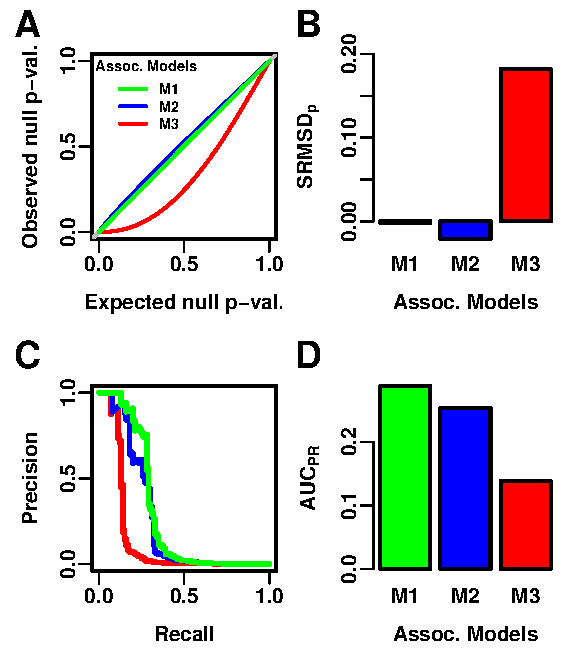
\includegraphics{sim-n1000-k10-f0.1-s0.5-g1/measures-illustration.pdf}
  \caption{
    {\bf Illustration of evaluation measures.}
    Three archetypal models illustrate our two complementary measures:
    M1 is well calibrated, M2 overfits slightly, and M3 does not model relatedness.
    \textbf{A.}
    QQ plot of p-values of ``null'' (non-causal) loci.
    M1 has uniform null p-values as desired (overlaps $y=x$).
    M2/M3 have null p-values larger/smaller than expected.
    \textbf{B.}
    $\rmsd$ (p-value Signed Root Mean Square Deviation) is a distance between the observed null p-values and their uniform expectations, negative if their median is larger than expected (closer to zero is better).
    \textbf{C.}
    Precision-Recall (PR) measure causal locus classification performance across thresholds without assuming calibrated p-values (higher is better).
    \textbf{D.}
    $\auc$ (Area Under the PR Curve) reflects power (higher is better).
  }
  \label{fig:measures_illustration}
\end{figure}

% PCA, LMM, PCs series
Both PCA and LMM were evaluated in each dataset including a number $r$ of PCs as fixed covariates, varying $r$ between 0 and 90, and every test was repeated 50 times.
Our overall statistical evaluation will be summarized first, followed by detailed evaluations in each datasets in the rest of the results.

First we describe the null p-value uniformity $|\rmsd|$ results (\cref{tab:human_sum_pcs}).
Here the sign of $\rmsd$ was ignored, so smaller is better and Wilcoxon paired 1-tailed tests were used to determine if a suboptimal distribution was significantly different.
For PCA, the optimal number of PCs $r$ is typically large across all datasets (up to $r=90$, the largest tested), but we found that much smaller ``min'' $r$ values often performed as well (numbers in parentheses in \cref{tab:human_sum_pcs}).
However, even the min $r$ values for PCA tended to be large on the family simulation and real datasets.
Most cases had a mean $|\rmsd| < 0.01$ (marked with asterisks), whose p-values are effectively calibrated.
Mean $|\rmsd| > 0.01$ (miscalibrated) PCA cases were observed on the family simulation and real datasets.
In contrast, for LMM, $r=0$ (no PCs) was always the optimal choice, and was always calibrated.
Lastly, comparing LMM with $r=0$ to PCA with its best $r$, LMM was either always significantly better or statistically tied to PCA.

\begin{table}[hb!]
  \centering
  %\scriptsize
  \caption{
    \textbf{Overview of PCA and LMM evaluation results}
  }
  \label{tab:human_sum_pcs}
  \csvreader[
  tabular = lc|ccc|ccc,
  separator = tab,
  table head = 
  % header row 1
  \toprule & Metric: & \multicolumn{3}{c|}{$|\rmsd|$} & \multicolumn{3}{c}{$\auc$} \\
  % header row 2
  \midrule & & \multicolumn{2}{c}{Best (min\textsuperscript{b}) PCs} & & \multicolumn{2}{c}{Best (min\textsuperscript{b}) PCs} & \\
  % header row 3
  Dataset & {Trait model\textsuperscript{a}} & PCA & LMM & {Best\textsuperscript{c}} & PCA & LMM & {Best\textsuperscript{c}} \\\midrule,
  late after last line = \\\bottomrule
  ]{../data/stats.txt}{}{\csvlinetotablerow}
  \begin{flushleft}
    \textsuperscript{a}FES: Fixed Effect Sizes, RC: Random Coefficients.\\
    \textsuperscript{b}Parentheses: smallest $r$ (number of PCs) whose distribution ($|\rmsd|$ or $\auc$) was not significantly different (Wilcoxon paired 1-tailed $p > 0.01$) from the $r$ with best mean value (if any). \\
    \textsuperscript{c}Tie if distributions of best PCA and LMM version (previous two columns) did not differ significantly (Wilcoxon paired 1-tailed $p > 0.01$).
    Result was always the same whether ``best'' or ``min'' (in parenthesis) cases were compared, except in two cases in parentheses.\\
    *$r$ for which mean $|\rmsd| < 0.01$ ($|\rmsd|$ columns only).
  \end{flushleft}
\end{table}

Next we turn to classification performance ($\auc$; \cref{tab:human_sum_pcs}).
For PCA, the best $r$ for $\auc$ was always smaller than the best $r$ for $|\rmsd|$, and also for the respective ``min'' $r$ comparisons.
Thus, for PCA there is often a tradeoff between calibrated p-values versus classification performance.
For LMM there is no such tradeoff, as $r=0$ (no PCs) resulted in $\auc$ distributions not significantly different from the best $r$ in all tests except two (the min $r$ was 2 for both 1000 Genomes simulation with FES trait and 1000 Genomes real dataset with RC trait).
Lastly, LMM with its best $r$ always had significantly greater $\auc$ distributions than PCA with its best $r$ except for one statistical tie.

\subsection{Evaluations in admixture simulations}

Now we look more closely at the results of every individual evaluation.
The $\rmsd$ and $\auc$ distributions for the first three admixture simulations and FES traits are in \cref{fig:rmsd-auc-sim}.
We repeated the evaluation with RC traits, which gave qualitatively similar results (\cref{fig:rmsd-auc-sim-rc}).

In the large admixture simulation, the $\rmsd$ of PCA is largest when $r=0$ (no PCs) and decreases rapidly to near zero at $r=3$, where it stays for up to $r=90$ (\cref{fig:rmsd-auc-sim}A).
Thus, PCA has calibrated p-values for $r \ge 3$, which is smaller than the theoretical optimum for this simulation of $r = K - 1 = 9$.
In contrast, the $\rmsd$ for LMM starts near zero for $r=0$, but becomes negative as $r$ increases (p-values are conservative).
The $\auc$ distribution of PCA is similarly worst at $r=0$, increases rapidly and peaks at $r = 3$, then decreases slowly for $r > 3$, while the $\auc$ distribution for LMM starts near its maximum at $r=0$, and decreases for larger $r$.
Although the $\auc$ distributions for LMM and PCA overlap considerably at each $r$, LMM with $r=0$ has significantly greater $\auc$ values than PCA with $r=3$ (\cref{tab:human_sum_pcs}).
However, qualitatively PCA closely matches LMM's performance in this simulation.
Both LMM and PCA are robust to extreme values of $r$.

\begin{figure}[bp!]
  \centering
  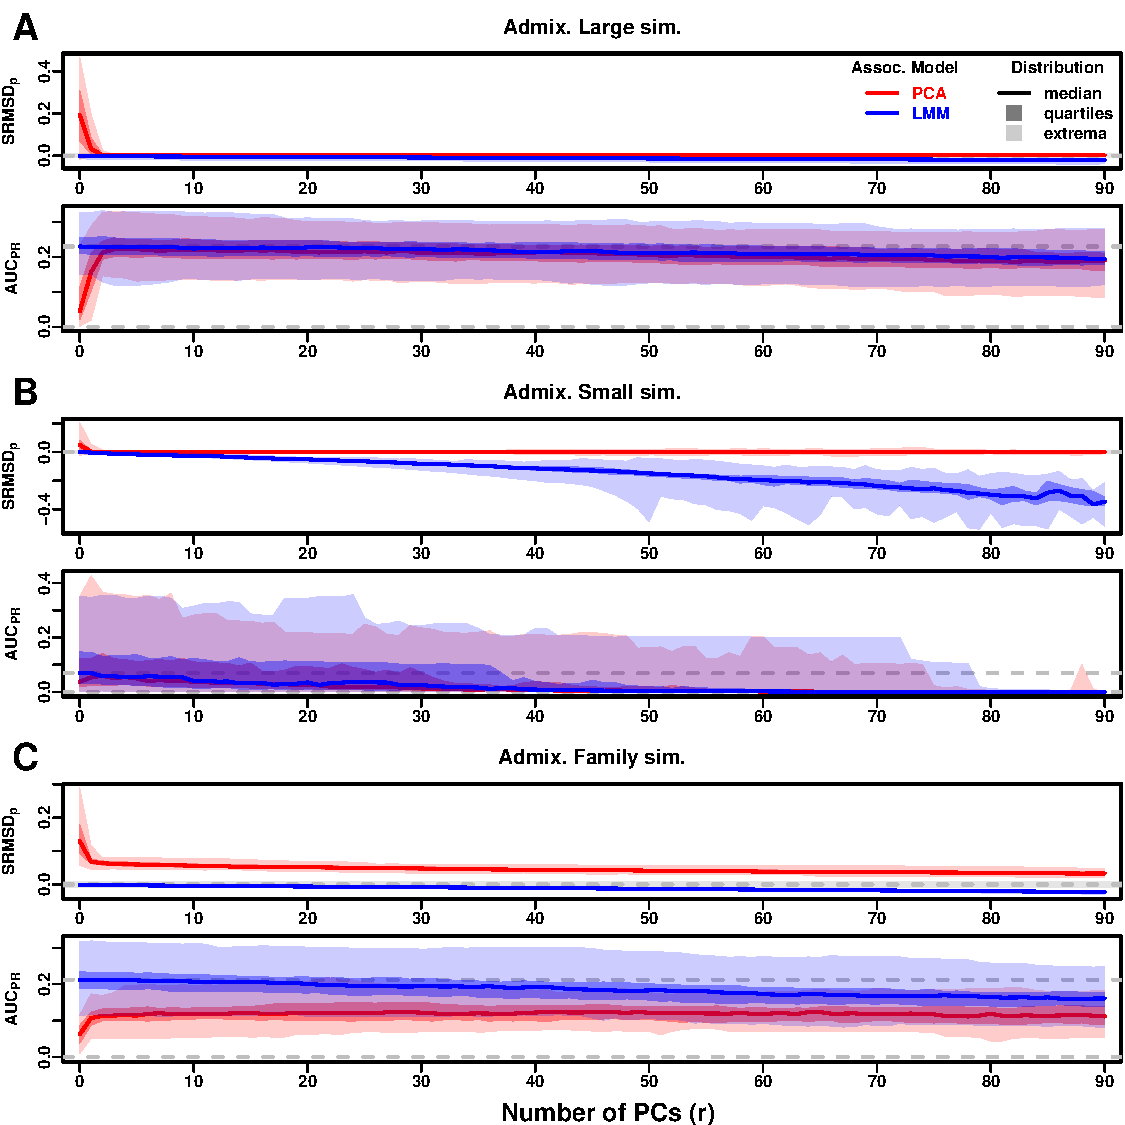
\includegraphics[width=\textwidth,height=\textheight,keepaspectratio]{fes/rmsd-auc-sim.pdf}
  \caption{
    {\small 
      {\bf Evaluations in admixture simulations.}
      Traits simulated from FES model.
      PCA and LMM models have varying number of PCs ($r \in \{0, ..., 90\}$ on x-axis), with the distributions (y-axis) of $\rmsd$ (top subpanel) and $\auc$ (bottom subpanel) for 50 replicates.
      Best performance is zero $\rmsd$ and large $\auc$.
      Zero values and maximum median $\auc$ values marked with horizontal gray dashed lines, and $|\rmsd| < 0.01$ band is marked with a light gray area.
      LMM always performs best with $r=0$, PCA with $r$ between 1-4.
      \textbf{A.}
      The large simulation has $n = 1,000$ individuals.
      \textbf{B.}
      The small simulation has $n = 100$ individuals, shows overfitting for large $r$.
      \textbf{C.}
      The family simulation has $n = 1,000$ individuals from a family with admixed founders and large numbers of close relatives from a realistic random 20-generation pedigree.
      PCA performs poorly compared to LMM: $\rmsd > 0$ for all $r$ and large $\auc$ gap.
    }
  }
  \label{fig:rmsd-auc-sim}
\end{figure}

The observed robustness to large $r$ led us to consider smaller sample sizes.
Our expectation is that a model with large numbers of parameters $r$ should overfit more as $r$ approaches the sample size $n$.
Rather than increase $r$ beyond 90, which is not done in practice, we reduce individuals to $n = 100$, which is small for typical association studies but may occur in studies of rare diseases, pilot studies, or other constraints.
To compensate for the loss of power due to reducing $n$, we also reduce the number of causal loci from 100 to $m_1 = 10$, (fixed ratio $n / m_1 = 10$) to increase per-locus effect sizes.
As expected, we found a large decrease in performance for both PCA and LMM as $r$ increases, with optimal performance attained near $r=1$ for PCA and $r=0$ for LMM (\cref{fig:rmsd-auc-sim}B).
Remarkably, LMM attains much larger negative $\rmsd$ values than in our other evaluations.
While LMM with $r=0$ is significantly better than PCA ($r=1$ to 4) in both metrics (\cref{tab:human_sum_pcs}), qualitatively the difference is negligible.

The family simulation adds a 20-generation random family to our admixture simulation.
Only the last generation is studied for association, which contains numerous siblings, first cousins, etc., with the initial admixture structure preserved by geographically-biased mating.
Previous work has reported, in limited settings, that PCA performs poorly with family structure, whereas LMM is formulated in terms of kinship so it is expected to perform better.
Our evaluation reveals a sizable gap in both metrics between LMM and PCA across all $r$ (\cref{fig:rmsd-auc-sim}C).
LMM again performs best with $r=0$ and achieves mean $|\rmsd| < 0.01$.
However, PCA does not achieve mean $|\rmsd| < 0.01$ at any $r$, and its best mean $\auc$ across $r$ is considerably worse than that of LMM.
Thus, LMM is conclusively superior to PCA, and the only calibrated model, when there is family structure.

\subsection{Evaluations in real human genotype datasets}

Next we repeat our evaluations with real human genotype data, which differs from our simulations in allele frequency distributions and more complex population structures with greater differentiation, numerous correlated subpopulations, and potential cryptic family relatedness.
We chose three datasets that span global human diversity and include both array and whole genome sequencing (WGS) genotyping platforms.
Loci in high linkage disequilibrium were removed to simplify our evaluation, and traits were simulated from these genotypes and FES (\cref{fig:rmsd-auc-real}) and RC (\cref{fig:rmsd-auc-real-rc}) models.

Human Origins has the greatest number and diversity of subpopulations.
The $\rmsd$ and $\auc$ distributions in this dataset and FES traits (\cref{fig:rmsd-auc-real}A) most resemble those from the family simulation (\cref{fig:rmsd-auc-sim}C).
In particular, while LMM with $r=0$ performed optimally (both metrics) and satisfies mean $|\rmsd| < 0.01$, PCA maintained $\rmsd > 0.01$ for all $r$ and its $\auc$ were all considerably smaller than the best $\auc$ of LMM.

\begin{figure}[bp!]
  \centering
  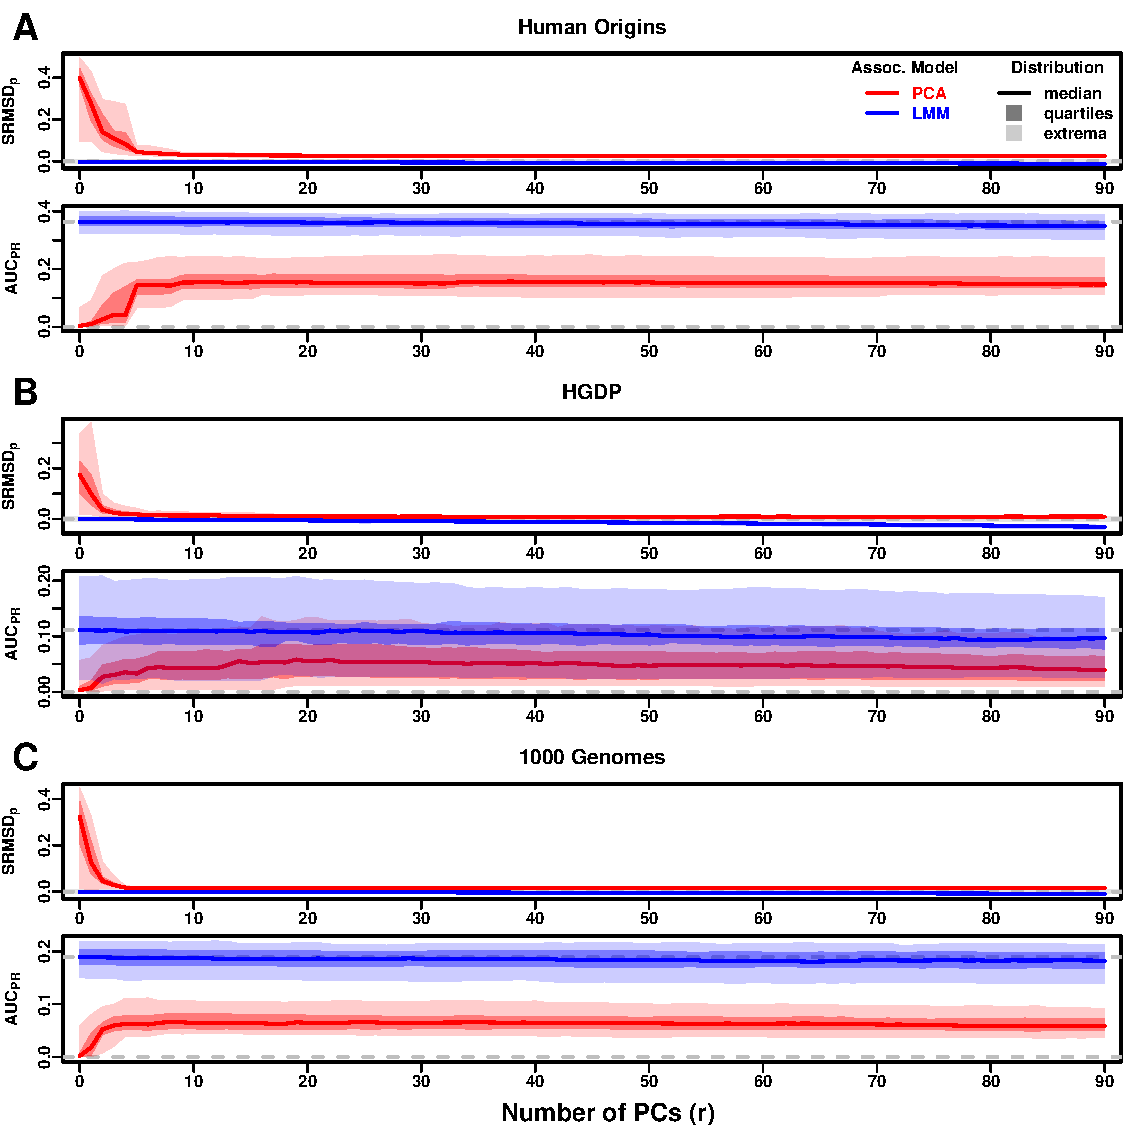
\includegraphics[width=\textwidth,height=\textheight,keepaspectratio]{fes/rmsd-auc-real.pdf}
  \caption{
    {\small 
      {\bf Evaluations in real human genotype datasets.}
      Traits simulated from FES model.
      Same setup as \cref{fig:rmsd-auc-sim}, see that for details.
      These datasets strongly favor LMM with $r = 0$ PCs over PCA, with distributions that most resemble the previous admixed family simulation.
      \textbf{A.}
      The Human Origins dataset.
      \textbf{B.}
      The Human Genome Diversity Panel (HGDP) dataset.
      \textbf{C.}
      The 1000 Genomes Project dataset.
    }
  }
  \label{fig:rmsd-auc-real}
\end{figure}

HGDP has the fewest individuals among real datasets, but compared to Human Origins it contains many more loci and low-frequency variants.
The $\rmsd$ and $\auc$ distributions (\cref{fig:rmsd-auc-real}B) are intermediate between the admixture and family simulations.
In particular, here both LMM ($r=0$) and PCA ($r \ge 31$) achieve mean $|\rmsd| < 0.01$ (p-values are calibrated).
However, there is a sizable $\auc$ gap between LMM and PCA.
Maximum $\auc$ values were lowest in HGDP compared to the two other real datasets.

1000 Genomes has the fewest subpopulations but largest number of individuals per subpopulation, and is WGS.
Thus, although this dataset is expected to have the simplest population structure among the real datasets, we find $\rmsd$ and $\auc$ distributions (\cref{fig:rmsd-auc-real}C) that again most resemble our earlier family simulation, with mean $|\rmsd| < 0.01$ for LMM only and large $\auc$ gaps between LMM and PCA.

Our results are qualitatively different for RC traits, which had smaller $\auc$ gaps between LMM and PCA (\cref{fig:rmsd-auc-real-rc}).
Maximum $\auc$ were smaller in RC compared to FES in Human Origins and 1000 Genomes, suggesting lower power for RC traits across association models.
Nevertheless, for RC traits we found LMM with $r=0$ significantly better than PCA for all metrics in the real datasets (\cref{tab:human_sum_pcs}).

\subsection{Evaluations in tree simulations fit to human data}

To better understand which features of the real datasets lead to the large differences in performance between LMM and PCA, we carried out additional simulations.
Human subpopulations are related roughly by trees, which induce the strongest correlations, so we fit trees to each real dataset and tested if data simulated from these trees could recapitulate our previous results (\cref{fig:kinship}).
These tree simulations also feature non-uniform ancestral allele frequency distributions, which recapitulated some of the skew for smaller minor allele frequencies of the real datasets (\cref{fig:kinship}C).

The $\rmsd$ and $\auc$ distributions for these tree simulations (\cref{fig:rmsd-auc-real-sim}) resembled our admixture simulation more than either the family simulation (\cref{fig:rmsd-auc-sim}) or real data results (\cref{fig:rmsd-auc-real}).
In all these simulations, both LMM with $r=0$ and PCA (various $r$) achieve mean $|\rmsd| < 0.01$ (\cref{tab:human_sum_pcs}).
The $\auc$ distributions of both LMM and PCA track closely as $r$ is varied, although there is a small gap resulting in LMM ($r=0$) besting PCA in all three simulations.
The results are qualitatively similar for the random coefficients trait model (\cref{fig:rmsd-auc-real-sim-rc,tab:human_sum_pcs}).
Overall, these tree simulations do not recapitulate the large LMM advantage over PCA observed in the real data results.

\begin{figure}[bp!]
  \centering
  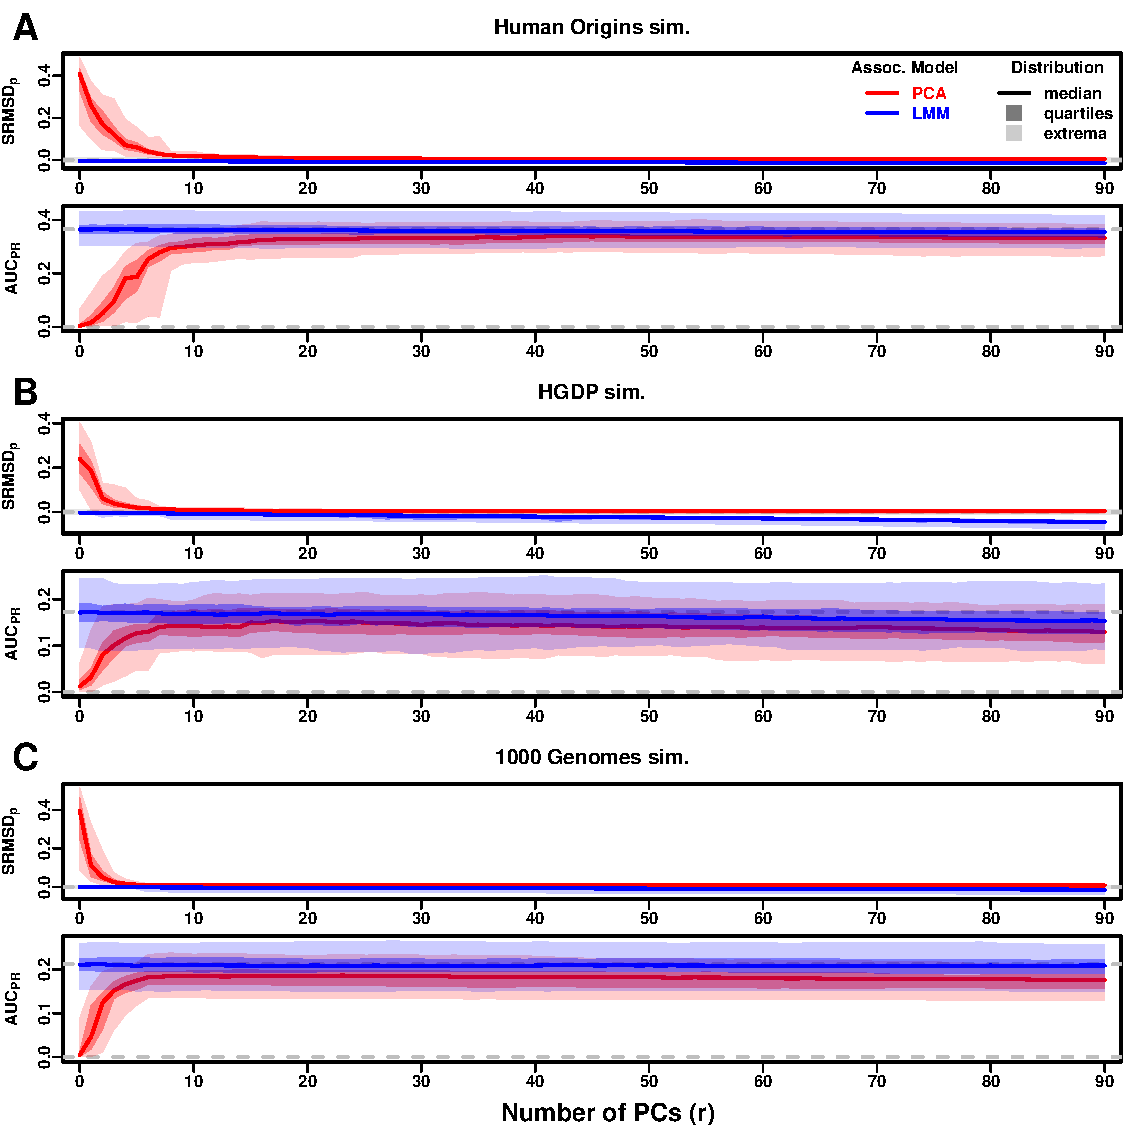
\includegraphics[width=\textwidth,height=\textheight,keepaspectratio]{fes/rmsd-auc-real-sim.pdf}
  \caption{
    {\small 
      {\bf Evaluations in tree simulations fit to human data.}
      Traits simulated from FES model.
      Same setup as \cref{fig:rmsd-auc-sim}, see that for details.
      These tree simulations, which exclude family structure by design, do not explain the large gaps in LMM-PCA performance observed in the real datasets.
      \textbf{A.}
      The Human Origins simulation.
      \textbf{B.}
      The Human Genome Diversity Panel (HGDP) simulation.
      \textbf{C.}
      The 1000 Genomes Project simulation.
    }
  }
  \label{fig:rmsd-auc-real-sim}
\end{figure}

\subsection{Estimated eigenvalues do not explain PCA performance}

A first-principles hypothesis for explaining PCA performance is the dimensionality of the population structure, since PCA assumes a low-dimensional genetic structure whereas LMM can model high-dimensional structures without overfitting.
We applied the Tracy-Widom test \citep{patterson_population_2006} with $p < 0.01$ to estimate the number of significant PCs in each dataset, which corresponds to the kinship matrix rank (\cref{fig:eigen}A).
These estimates slightly underestimated the true dimensionality of our simulations (\cref{tab:human_sum}), but agree that the family simulation has the greatest rank by far, and estimates greater ranks for the real datasets than their respective tree simulations.
However, these estimated ranks do not differentiate datasets with good PCA performance from those with poor performance, particularly between the real and tree simulations, which span a similar range of ranks.
Moreover, the 1000 Genomes rank estimate is lower than 90, yet PCA performed poorly for all $r \ge 90$ numbers of PCs tested (\cref{fig:rmsd-auc-real}).
Performance might also depend on the sample size, but these datasets do not differ greatly in size (at most 3$\times$, excluding the small simulation), while our analysis does not reveal a line that separates datasets by PCA performance.

We also compared eigenvalues across datasets expressed as variance explained to facilitate comparisons across datasets (\cref{fig:eigen}C).
The top eigenvalue explained a proportion of variance proportional to \Fst (\cref{tab:human_sum}), but the rest of the top 10 eigenvalues show no clear differences between datasets, except the small simulation had larger variances explained per eigenvalue (as expected since it has fewer eigenvalues).
Lastly, we compared cumulative variance explained versus eigenvalue rank fraction (\cref{fig:eigen}B).
Each dataset has a different starting point, but all increase almost linearly from there until they reach 1, except the family simulation has much greater variance explained by mid-rank eigenvalues.
There is again no clear separation between real datasets (where PCA performed poorly) from the corresponding tree simulations (where PCA performed relatively well).

\subsection{Local kinship explains PCA performance}

Local kinship, which is relatedness due to family structure excluding population structure, is the presumed cause of the LMM to PCA performance gap observed in real datasets but not their tree simulation counterparts.
Instead of inferring local kinship through increased dimensionality, as attempted in the last section, here we measure it directly using the KING-robust estimator \citep{manichaikul_robust_2010}.
As expected, we observe more large local kinship values in the real datasets and the family simulation compared to the admixture and tree simulations (\cref{fig:king}).
However, for real datasets this distribution depends on the subpopulation structure, since locally related pairs are most likely in the same subpopulation while pairs between subpopulations tend to be negative for this estimator.
Therefore, the only comparable curve to each real dataset is their corresponding tree simulation, which matches subpopulation structure.

\begin{figure}[bp!]
  \centering
  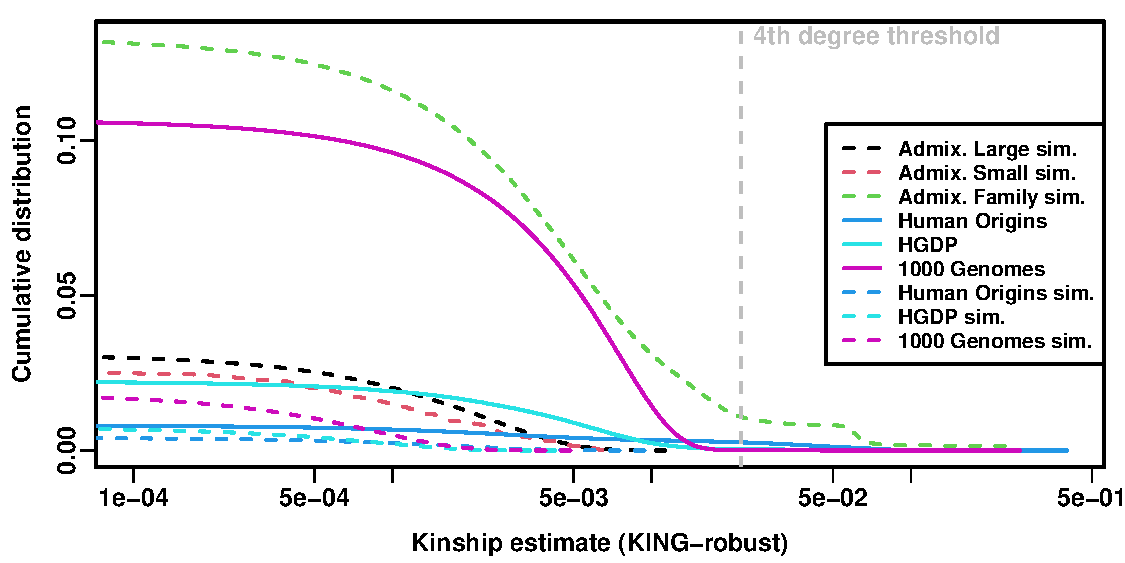
\includegraphics[width=\textwidth]{king_log-x.pdf}
  \caption{
    {\bf Local kinship estimate distribution.}
    Curves are the complementary cumulative distribution of all lower triangular kinship matrix values from the KING-robust estimator.
    Self kinship is excluded.
    Note log scale of x-axis; negative estimates are counted but not shown.
    Most values in all datasets are below the 4th degree relative threshold value.
    Each real dataset has a greater cumulative than its tree simulations.
  }
  \label{fig:king}
\end{figure}

In all real datasets we identified highly related individual pairs with kinship above the 4th degree relative threshold of 0.022 \citep{manichaikul_robust_2010, conomos_model-free_2016}.
However, these highly related pairs are vastly outnumbered by pairs who are less related but have greater than zero kinship (\cref{fig:king}).
Non-zero kinship can be inferred using the tree simulations' distribution as a null, which allowing for a small fraction of false positives suggests kinship above 0.001 or 0.01 for these datasets.

To try to improve PCA performance, we removed 4th degree relatives, which reduced sample sizes between 5\% and 10\% (\cref{tab:king_cutoff}).
Only $r=0$ for LMM and $r=20$ for PCA were tested, as these performed well in our earlier evaluation.
Only FES traits were tested, which earlier showed a large performance gap between association models.
LMM significantly outperforms PCA in all these cases (Wilcoxon paired 1-tailed $p < 0.01$; \cref{fig:king_cutoff}).
Notably, PCA still had miscalibrated p-values in Human Origins and 1000 Genomes ($|\rmsd| > 0.01$).
Otherwise, $\auc$ and $\rmsd$ ranges were similar here as in the test with all individuals.
Therefore, the small number of highly related individual pairs had a negligible effect in PCA performance, so the larger number of more distantly related pairs explain the poor PCA performance compared to LMM in the real datasets.

\begin{figure}[bp!]
  \centering
  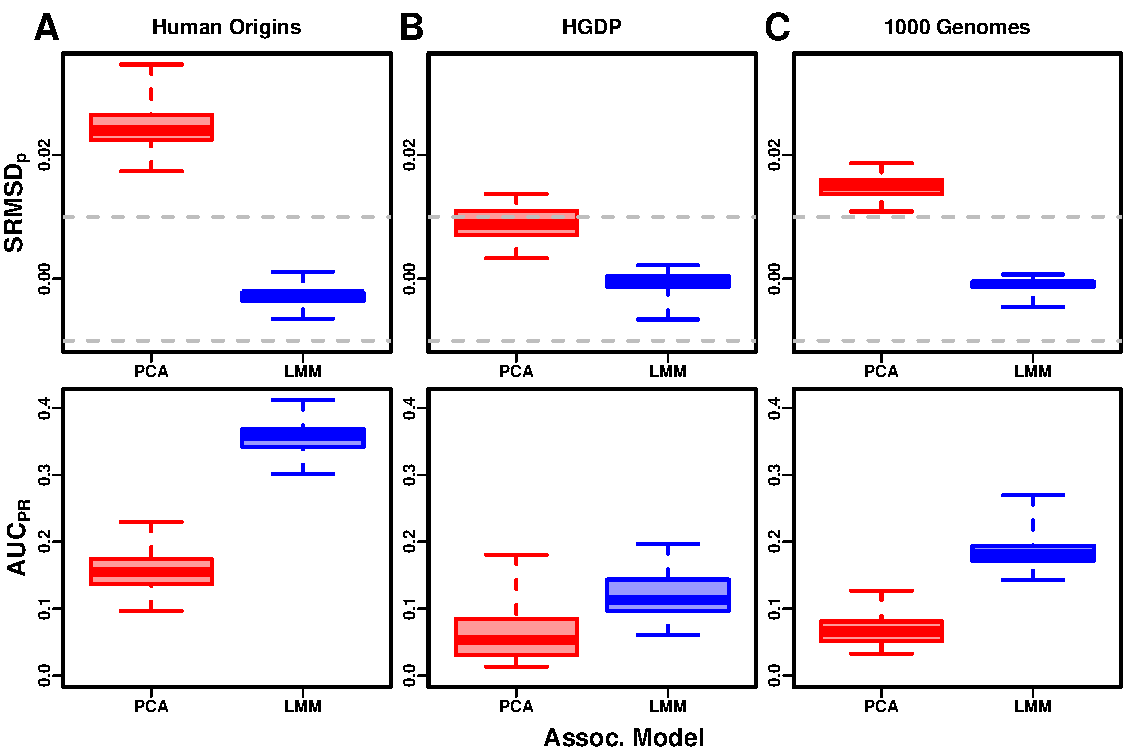
\includegraphics[width=\textwidth]{fes/rmsd-auc_king-cutoff-4.pdf}
  \caption{
    {\bf LMM and PCA performance in real datasets excluding 4th degree relatives.}
    LMM had $r=0$ PCs and PCA had $r=20$.
    FES traits only.
    Each dataset is a column, rows are metrics.
    First row has $|\rmsd| < 0.01$ band marked with dashed gray lines.
  }
  \label{fig:king_cutoff}
\end{figure}


\section{Discussion}

Our evaluations conclusively determined that LMM without PCs performs better than PCA (for any number of PCs) across all scenarios, including all real and simulated genotypes and two trait simulation models.
Although the addition of a few PCs does not greatly hurt the performance of LMM (except for small sample sizes), such additions rarely improved performance (\cref{tab:human_sum_pcs}), which agrees with previous observations \citep{liu_controlling_2011} but contradicts others \citep{zhao_arabidopsis_2007, price_new_2010}.
Our findings make sense since PCs are the eigenvectors of the kinship matrix used to model the random effects, so including both is redundant.

Previous studies had found that PCA was better calibrated than LMM in a hypothetical setting, namely unusually differentiated markers \citep{price_new_2010, wu_comparison_2011, yang_advantages_2014}, which as simulated are an artificial scenario not based on a population genetics model, and are otherwise believed to be unusual \citep{sul_mixed_2013, price_response_2013}.
Our evaluations on real human data, which contain such loci in relevant proportions if they exist, do not replicate that result.
The presence of cryptic relatedness strongly favors LMM, an advantage that probably always outweighs this potential PCA benefit in real datasets.

Relative to LMM, the behavior of PCA fell between two extremes.
When PCA performed well, there was a small number of PCs with both $\rmsd$ near zero and $\auc$ near that of LMM without PCs.
Conversely, when PCA performed poorly, no number of PCs had either acceptably low $\rmsd$ or acceptably large $\auc$.
PCA performed well in the admixture simulations (without families, both trait models), real human genotypes with RC traits, and, to a lesser extent, the tree simulations (both trait models).
Conversely, PCA performed poorly in the admixed family simulation (both trait models) and the real human genotypes with FES traits.

PCA assumes that genetic structure is low-dimensional, whereas LMM can handle high-dimensional structures.
Thus, PCA performs well in the admixture simulation, which is explicitly low-dimensional (see Models and Methods), and our tree simulations, which had few nodes with long branches so a low-dimensional approximation suffices.
Conversely, PCA performs poorly under family structure because its kinship matrix is high-dimensional (\cref{fig:eigen}).
One theoretical inconvenience is that true kinship matrices are always full rank: for example, an unstructured population has a kinship matrix of $\mathbf{I}/2$, whose eigenvalues are all equal to $1/2$ (none are zero).
Population structure induces an unbalanced eigenvalue distribution with few large eigenvalues (\cref{fig:eigen}), so in practice dimensionality is given by the number of eigenvalues above some small threshold.
Estimating the dimensionality of real datasets is challenging because estimated kinship matrices have noisy eigenvalues with biased distributions.
We used the Tracy-Widom test to estimate dimensionality \citep{patterson_population_2006}, which slightly underestimates the dimensionality of our simulations (an expected loss of power to detect eigenvalues which are also less important in our association tests).
Estimated eigenvalues alone do not predict when PCA will perform poorly.
Estimated local kinship finds considerable cryptic relatedness in all real human datasets, better explaining why LMM outperforms PCA there.
The trait model also influences the relative performance of PCA, so genotype-only eigenvalues or local kinship alone do not tell the full story.

The real human genotype results, which are the most relevant in practice, suggests that PCA is at best underpowered relative to LMMs, and at worst miscalibrated regardless of the numbers of PCs included.
Among our simulations, such poor performance occurred only in the admixed family simulation.
Local kinship estimates reveal considerable family relatedness in the real datasets absent in the corresponding tree simulations.
Admixture is absent in our tree simulations, but our simulations and theory show that admixture is handled well by PCA.
Hundreds of close relative pairs have been identified in 1000 Genomes \citep{gazal_high_2015, al-khudhair_inference_2015, fedorova_atlas_2016, schlauch_identification_2017}, but their removal does not improve PCA performance sufficiently in our tests, so the larger number of more distantly related pairs are PCA's most serious obstacle in practice.
Distant relatives are expected to be numerous in any large human dataset \citep{henn_cryptic_2012, shchur_number_2018}.
Furthermore, our FES trait tests show that the challenges of cryptic relatedness are exacerbated when rarer variants have larger coefficients.
Overall, the high dimensionality induced by cryptic relatedness is the key challenge for PCA association in modern datasets that is readily overcome by LMM.

Our tests also found PCA robust to large numbers of PCs, far beyond the optimal choice, agreeing with previous anecdotal observations \citep{price_principal_2006, kang_variance_2010}, in contrast to using too few PCs for which there is a large performance penalty.
The exception was the small sample size simulation, where only small numbers of PCs performed well.
In contrast, LMM is simpler since there is no need to choose the number of PCs.
However, an LMM with a large number of covariates may have conservative p-values (as we observed for LMM with large numbers of PCs), a weakness of the asymptotic test used by this LMM that can be overcome with a more accurate test such as the t-test used by PCA.
Simulations or post hoc evaluations remain crucial (for any association model) to ensure that statistics are calibrated.

The largest limitation of our work is that we only considered quantitative traits.
We noted that previous evaluations involving case-control traits tended to report PCA-LMM ties or mixed results, but also tended to employ low-dimensional simulations which do not feature cryptic relatedness (\cref{tab:lit}).
An additional concern in these studies is case-control ascertainment bias, which appears to affect LMMs more severely although recent work appears to solve this problem \citep{yang_advantages_2014, zhou_efficiently_2018}.
Future work should aim to ask these questions in the context of our new genotype simulations and real datasets, to ensure that previous results were not biased in favor of PCA by employing unrealistic low-dimensional genotype simulations, or by not simulating large coefficients for rare variants that are predicted for diseases by various selection models.

Overall, our results lead us to always recommend LMM over PCA for association studies.
Although PCA offer flexibility and speed compared to LMM, in practice much additional work is required to ensure that PCA is adequate, including removal of close relatives (lowering sample size and wasting resources) followed by simulations or other evaluations of statistics, and even then there is no guarantee that PCA will perform nearly as well as LMM, in terms of both type I error control and power.
The large numbers of distant relatives expected of any real dataset all but ensures that PCA will perform poorly in practice compared to LMM for association studies.
Our findings also suggest that related applications such as polygenic models may enjoy gains in power and accuracy by employing an LMM instead of PCA to model relatedness \citep{rakitsch_lasso_2013,qian_fast_2020}.
PCA remains indispensable across population genetics, from visualizing population structure and performing quality control to its deep connection to admixture models, but the time has come to limit its use in association testing in favor of LMM or other, richer models capable of modeling all forms of relatedness.

\section{Models and Methods}

\subsection{Models for genetic association studies}

Here we describe the complex trait and kinship models that motivate PCA and LMM.
The derivations of PCA and LMM from the general quantitative trait model are similar to previous presentations \citep{astle_population_2009, hoffman_correcting_2013}, but we emphasize the kinship model for random genotypes as crucial for these connections, and clearly distinguish the true kinship matrix from its biased common estimator \citep{ochoa_estimating_2021, ochoa_human}.

\subsubsection{The complex trait model and PCA approximation}

Let $\xij \in \{ 0, 1, 2 \}$ be the genotype at the biallelic locus $i$ for individual $j$, which counts the number of reference alleles.
Suppose there are $n$ individuals and $m$ loci,
$\mathbf{X} = ( \xij )$ is their $m \times n$ genotype matrix, and
$\mathbf{y}$ is the length-$n$ (column) vector of individual trait values.
The additive linear model for a quantitative (continuous) trait is:
\begin{equation}
  \label{eq:trait}
  \mathbf{y}
  =
  \mathbf{1} \alpha + \mathbf{X}^\intercal \boldsymbol{\beta} + \boldsymbol{\epsilon}
  ,
\end{equation}
where
$\mathbf{1}$ is a length-$n$ vector of ones,
$\alpha$ is the scalar intercept coefficient,
$\boldsymbol{\beta}$ is the length-$m$ vector of locus coefficients,
$\boldsymbol{\epsilon}$ is a length-$n$ vector of residuals,
and $\intercal$ denotes matrix transposition.
The residuals follow $\epsilon_j \sim \text{Normal}(0, \sigma^2)$ independently per individual $j$, for some $\sigma^2$.
For simplicity, non-genetic covariates are omitted from this model (and the PCA and LMM counterparts) but are trivial to include without changing any of our theoretical results.

Current datasets have millions of loci $m$ while most have many fewer than a million individuals $n$.
The full model above cannot be fit for $m \ge n$, as there are more parameters ($m+2$, the length of $\boldsymbol{\beta}$, $\alpha$, $\sigma^2$) than samples ($n$, the length of $\mathbf{y}$).
The PCA model with $r$ PCs approximates the full model fit at a single locus $i$:
\begin{equation}
  \label{eq:pca_gwas}
  \mathbf{y}
  =
  \mathbf{1} \alpha + \mathbf{x}_i \beta_i + \mathbf{U}_r \boldsymbol{\gamma}_r + \boldsymbol{\epsilon}
  ,
\end{equation}
where $\mathbf{x}_i$ is the length-$n$ vector of genotypes at locus $i$ only,
$\beta_i$ is the locus coefficient,
$\mathbf{U}_r$ is an $n \times r$ matrix of PCs, and
$\boldsymbol{\gamma}_r$ is the length-$r$ vector of PC coefficients.
This approximation follows from the singular value decomposition of the genotype matrix:
$\mathbf{X}^\intercal = \mathbf{U} \mathbf{D} \mathbf{V}^\intercal$,
where
$\mathbf{U}$ is an $n \times n$ matrix of left singular vectors of $\mathbf{X}$,
$\mathbf{V}$ is an $m \times n$ matrix of its right singular vectors, and
$\mathbf{D}$ is an $n \times n$ diagonal matrix of its singular values.
Thus, the full model has
$\mathbf{X}^\intercal \boldsymbol{\beta} = \mathbf{U} \boldsymbol{\gamma}$,
where
$\boldsymbol{\gamma} = \mathbf{D} \mathbf{V}^\intercal \boldsymbol{\beta}$ is a length-$n$ vector.
The approximation consists of replacing $\mathbf{U} \boldsymbol{\gamma}$ (the full set of $n$ left singular vectors and their coefficients) with $\mathbf{U}_r \boldsymbol{\gamma}_r$ (the top $r$ singular vectors only), which is the best rank-$r$ approximation of the genotypes \citep{jolliffe_principal_2002}. % Property A5, pg 47 of PDF
Thus, PCs approximate the polygenic effect of the whole genome, and assumes that locus $i$ being tested does not contribute greatly to this signal.

The null hypothesis of $\beta_j = 0$ (no association) is evaluated with a standard regression t-test, yielding a two-sided p-value.
Some PCA implementations trade this t-test for an asymptotic $\chi^2$ test, which requires the number of parameters to be much smaller than the number of individuals.

\subsubsection{Kinship model for genotypes}

To better motivate the most common PC estimator for genotype data, and to connect PCA to LMM, consider the kinship model for random genotypes obeying
$$
\E[ \xij | T ]
=
2 \pit,
\quad\quad
\Cov( \xij, \xij[k] | T )
=
4 \pit ( 1 - \pit ) \kt,
$$
where $T$ is the ancestral population (on which random variables are conditioned upon, usually the most recent common ancestor population), \pit is the ancestral allele frequency of locus $i$, and \kt is the kinship coefficient between individuals $j$ and $k$ \citep{malecot_mathematiques_1948, wright_genetical_1951, jacquard_structures_1970}.
Thus, the genotype matrix can be theoretically standardized using \pit as
$$
\mathbf{X}_S
=
\left(
  \frac{
    \xij - 2 \pit
  }{
    \sqrt{4 \pit \left( 1 - \pit \right)}
  }
\right)
,
$$
which results in the kinship estimator
$$
\E
\left[
\frac{1}{m}
\mathbf{X}_S^\intercal
\mathbf{X}_S
\right]
=
\mathbf{\Phi}^T
,
$$
where $\mathbf{\Phi}^T = ( \kt )$ is the $n \times n$ kinship matrix (do not confuse the ancestral population superscript $T$ with the matrix transposition symbol $\intercal$).
Replacing $\mathbf{X}$ with the standardized $\mathbf{X}_S$ in the trait model of \cref{eq:trait} results in an equivalent model that differs only by a linear transformation.
Thus, starting from standardized genotypes, the PCs of interest are equal in expectation to the top eigenvectors of the kinship matrix.

\subsubsection{Estimation of PCs from genotype data}

In practice, the matrix of PCs $\mathbf{U}_r$ in \cref{eq:pca_gwas} is calculated from an estimate of $\mathbf{X}_S$, namely
\begin{equation*}
  \mathbf{\hat{X}}_S
  =
  \left(
    \frac{
      \xij - 2 \pith
    }{
      \sqrt{4 \pith \left( 1 - \pith \right)}
    }
  \right)
  ,
\end{equation*}
where \pit is replaced by the estimate
$
\pith = \frac{1}{2n} \sum_{j = 1}^n \xij,
$
and results in the kinship estimate
\begin{equation}
  \label{eq:kinship_std}
  \mathbf{\hat{\Phi}}^T
  =
  \frac{1}{m}
  \mathbf{\hat{X}}_S^\intercal
  \mathbf{\hat{X}}_S
  .
\end{equation}
This kinship estimate and minor variants are also employed in all modern LMMs \citep{yang_gcta:_2011}.
However, this kinship estimator has a complex bias that differs for every individual pair \citep{ochoa_estimating_2021, ochoa_human}.
Nevertheless, in PCA and LMM these biased estimates perform as well as using unbiased estimates, an observation that will be explored in future work (data not shown).
%[TODO: cite BIAS GWAS]

\subsubsection{Connection between PCs and ancestry proportions}

Here we show that association using global ancestry proportions as covariates is equivalent in expectation to using PCs under the admixture model, which has been demonstrated empirically before \citep{alexander_fast_2009, zhou_strong_2016} and is the basis of recent admixture inference models \citep{zheng_eigenanalysis_2016,cabreros_likelihood-free_2019}.
We shall assume the standard individual-specific admixture model \citep{pritchard_inference_2000, alexander_fast_2009}.
There are $K$ subpopulations and every individual $j$ draws a proportion $q_{ju}$ of its alleles from subpopulation $S_u$, so ancestry proportions are non-negative and sum to one for every individual $j$.
Each subpopulation $S_u$ has an allele frequency $p_i^{S_u}$ at locus $i$, and thus the individual-specific allele frequency $\pi_{ij}$ is the mean subpopulation allele frequencies weighted by the ancestry proportions:
\begin{equation}
  \label{eq:admix}
  \pi_{ij} = \sum_{u=1}^K q_{ju} p_i^{S_u}.
\end{equation}
Genotypes are the sum of alleles drawn independently from this frequency: $\xij | \pi_{ij} \sim \text{Binomial}(2, \pi_{ij})$.
Thus, the rowspace of $\mathbf{X}$ equals in expectation that of $(\pi_{ij})$, which by \cref{eq:admix} is the same as the rowspace of the $n \times K$ admixture proportions matrix $\mathbf{Q} = (q_{ju})$.
Therefore, the top $K$ PCs span the rowspace of the genotypes.
Since associations include an intercept term ($\mathbf{1} \alpha$ in \cref{eq:pca_gwas}), estimated PCs are orthogonal to $\mathbf{1}$ (note $\mathbf{\hat{\Phi}}^T \mathbf{1} = \mathbf{0}$ because $\mathbf{\hat{X}}_S \mathbf{1} = \mathbf{0}$), and the sum of rows of $\mathbf{Q}$ sums to one, then only $K-1$ PCs (plus intercept) are needed to span the rowspace of this admixture model.

\subsubsection{The LMM approximation}

The LMM is another approximation to the complex trait model in \cref{eq:trait}, given by
\begin{equation}
  \label{eq:lmm_gwas}
  \mathbf{y}
  =
  \mathbf{1} \alpha + \mathbf{x}_i \beta_i + \mathbf{s} + \boldsymbol{\epsilon}
  ,
\end{equation}
which compared to PCA (\cref{eq:pca_gwas}) replaces the PCs $\mathbf{U}_r \boldsymbol{\gamma}_r$ with the random effect $\mathbf{s}$, which is a length-$n$ vector drawn from \citep{sul_population_2018}
$$
\mathbf{s} \sim \text{Normal} \left( \mathbf{0}, \sigma^2_s \mathbf{\Phi}^T \right),
$$
where $\mathbf{\Phi}^T$ is the kinship matrix and $\sigma^2_s$ is a variance factor.
This model is derived from treating the standardized genotype matrix $\mathbf{X}_S$ as random, so the standardized genetic effect
$\mathbf{X}_S^\intercal \boldsymbol{\beta}_S$
has mean zero and covariance
$$
\Cov \left( \mathbf{X}_S^\intercal \boldsymbol{\beta}_S \right)
=
|| \boldsymbol{\beta}_S ||^2 \mathbf{\Phi}^T
.
$$
The above $\mathbf{s}$ satisfies those equations with $\sigma^2_s = || \boldsymbol{\beta}_S ||^2$.
Thus, PCA is the fixed model equivalent of LMM under the additional approximation that only the top $r$ eigenvectors are used, whereas LMM uses all eigenvectors (see next subsection).

LMM has fewer parameters to fit compared to PCA: ignoring the shared terms in \cref{eq:pca_gwas} and \cref{eq:lmm_gwas}, PCA has $r$ parameters to fit (length of $\boldsymbol{\gamma}$), whereas LMMs fit only one ($\sigma^2_s$).
Therefore, PCA may overfit more than LMM---and thus lose power---when $r$ is very large and the sample size small.
Statistical significance in LMMs has been performed with various tests, including F tests, score tests, and Wald tests.

\subsubsection{Connection between LMM and PCA}

The LMM of \cref{eq:lmm_gwas} can be written to better resemble PCA of \cref{eq:pca_gwas}, as \citep{astle_population_2009, hoffman_correcting_2013}:
\begin{equation}
  \label{eq:lmm_gwas_evd}
  \mathbf{y}
  =
  \mathbf{1} \alpha + \mathbf{x}_i \beta_i + \mathbf{U} \boldsymbol{\gamma}_\text{LMM} + \boldsymbol{\epsilon}
  , \quad\quad
  \boldsymbol{\gamma}_\text{LMM} = \sigma_s \boldsymbol{\Lambda}^{1/2} \mathbf{r}
  ,
\end{equation}
where $\mathbf{U}$ is the PCs matrix (all $n$ of them), $\boldsymbol{\Lambda}$ is the diagonal eigenvalue matrix of the kinship matrix ($\mathbf{\Phi}^T = \mathbf{U} \boldsymbol{\Lambda} \mathbf{U}^\intercal$), and $\mathbf{r} \sim \text{Normal}(\mathbf{0},\mathbf{I})$.
The connection follows since $\mathbf{s} = \sigma_s \mathbf{U} \boldsymbol{\Lambda}^{1/2} \mathbf{r}$ satisfies
$$
\mathbf{s} \sim \text{Normal} \left( \mathbf{0}, \left( \sigma_s \mathbf{U} \boldsymbol{\Lambda}^{1/2} \right) \left( \sigma_s \mathbf{U} \boldsymbol{\Lambda}^{1/2} \right)^\intercal \right)
= \text{Normal}( \mathbf{0}, \sigma_s^2 \mathbf{\Phi}^T ),
$$
which itself follows from the affine transformation property of multivariate normal distributions.
$\mathbf{U}$ also equals in the limit the right singular vectors of the standardized genotype matrix $\mathbf{X}_S = \mathbf{V}_S \mathbf{D}_S \mathbf{U}_S^\intercal$, which is how we originally motivated PCA, since
$$
\frac{1}{m} \mathbf{X}_S^\intercal \mathbf{X}_S
%= \frac{1}{m} \mathbf{U}_S \mathbf{D}_S \mathbf{V}_S^\intercal \mathbf{V}_S \mathbf{D}_S \mathbf{U}_S^\intercal
= \mathbf{U}_S \mathbf{\Lambda}_S \mathbf{U}_S^\intercal
\toas
\mathbf{U} \mathbf{\Lambda} \mathbf{U}^\intercal
=
\mathbf{\Phi}^T
$$
since $\mathbf{V}_S$ is orthonormal, and where $\mathbf{\Lambda}_S = \frac{1}{m} \mathbf{D}_S^2$.

Therefore, when the kinship matrix is low-dimensional, the LMM fits the same low-dimensional space as PCA, except that the coefficients $\boldsymbol{\gamma}_\text{LMM}$ are shrunk by the likelihood model, whereas PCA's $\boldsymbol{\gamma}_r$ are unconstrained.
On the other hand, when the kinship matrix is high-dimensional then LMM fits this space better than PCA with any number of PCs $r$, since large $r$ will overfit.

\subsection{Simulations}

Below we use the following notation.
Let $\f{B}{A}$ denote the inbreeding coefficient of a subpopulation $A$ from another subpopulation $B$ ancestral to $A$.
In the special case of the \textit{total} inbreeding of $A$, $\ft[A]$, $T$ is an overall ancestral population (ancestral to every subpopulation and/or individual under consideration, such as the most recent common ancestor population).

\subsubsection{Genotype simulation from the admixture model}

We consider three admixture simulation scenarios: Large, Small, and Family.
The basic admixture model is as described previously \citep{ochoa_fst1, ochoa_estimating_2021}.

Large and Family have $n = 1,000$ individuals, while Small has $n = 100$.
The number of loci is $m = 100,000$.
Individuals are admixed from $K = 10$ intermediate subpopulations, or ancestries.
Each subpopulation $S_u$ ($u \in \{ 1, ..., K \}$) lies at coordinate $u$ and has an inbreeding coefficient $\ft[S_u] = u \tau$ for some $\tau$.
Ancestry proportions $q_{ju}$ for individual $j$ and subpopulation $S_u$ arise from a random walk model on the given 1-dimensional geography with spread $\sigma$, and the free parameters $\tau$ and $\sigma$ are fit to result in $\Fst = 0.1$ and mean kinship $\bar{\theta}^T = 0.5 \Fst$ for the admixed individuals, as before \citep{ochoa_estimating_2021}.

Random allele frequencies and genotypes are drawn from this hierarchical model:
\begin{align*}
  \pit
  &\sim
    \text{Uniform}( 0.01, 0.5 )
    , \\
  p_i^{S_u} | \pit
  &\sim
    \text{Beta} \left(
    \pit \left( \frac{1}{ \ft[S_u] } - 1 \right),
    \left( 1 - \pit \right) \left( \frac{1}{ \ft[S_u] } - 1 \right)
    \right)
    , \\
  \pi_{ij}
  &=
    \sum_{u = 1}^K q_{ju} p_i^{S_u}
    , \\
  \xij | \pi_{ij}
  &\sim
    \text{Binomial}(2, \pi_{ij})
    .
\end{align*}
Briefly, ancestral allele frequencies \pit are drawn independently per locus $i$.
Subpopulation allele frequencies $p_i^{S_u}$ are drawn independently for each $S_u$ from the Balding-Nichols distribution with mean \pit and variance $\pit \left( 1 - \pit \right) \ft[S_u]$ \citep{balding_method_1995}.
Lastly, the individual-specific allele frequencies $\pi_{ij}$ and genotypes \xij are as in the admixture model (\cref{eq:admix}).
Fixed loci ($i$ where $\xij = 0$ for all $j$, or $\xij = 2$ for all $j$) are drawn again from the model, starting from \pit, iterating until no loci are fixed.
Each replicate draws a new genotype matrix starting from \pit.

\subsubsection{Genotype simulation from random admixed families}

We simulated a pedigree with admixed founders that features:
(1) strict avoidance of close relatives when pairing individuals;
(2) favoring close pairs in their 1-dimensional geography, which helps preserve the population structure by preferentially pairing individuals with similar admixture proportions (a form of assortative mating); and
(3) many generations, resulting in a distribution of close and distant relatives.

The 20 generations are drawn iteratively.
Generation 1 has individuals from the large admixture simulation.
These individuals are ordered by the 1-dimensional geography of the admixture scenario.
The local kinship matrix measures the pedigree relatedness; in the first generation, everybody is locally unrelated and outbred.
Individuals are randomly assigned to male or female with equal probability.

The children of the previous generation are the parents in the next generation, paired iteratively as follows.
From the pool of available males, one is picked randomly and is paired with the nearest female that is not a second cousin or closer relative (local kinship must be $< 1/4^3$); males that are not pairable are removed from the pool of available males.
Pairing stops when there are no more available males or females.

Next, a random number of children per pair is constructed to yield a desired population size $n$ and a minimum family size of $n_m=1$, as follows.
Let $n_f$ the be number of families (paired parents) in the current generation, then the number of additional children (beyond the minimum) is drawn from a Poisson distribution with parameter $n/n_f - n_m$.
Although the mean population size is $n$ as desired, the random sample may deviate from this target size.
Let $\delta$ be the difference between desired and current population sizes.
If $\delta > 0$, then $\delta$ random families are incremented by 1.
If $\delta < 0$, then $|\delta|$ random families with at least $n_m+1$ children are decremented by 1.
If $|\delta|$ exceeds the number of families, all families are incremented or decremented as needed and the process is iterated.
Children are assigned sex randomly, and are reordered by the average coordinate of their parents.

Children draw alleles from their parents independently per locus.
A new random pedigree was drawn for each replicate, as well as new founder genotypes from the admixture model.

\subsubsection{Genotype simulation from a tree model}

This variant of the admixture model draws subpopulations allele frequencies from a hierarchical model parametrized by a tree.
The ancestral population $T$ is at the root of the tree, and each node is a subpopulation $S_w$ indexed ($w$) arbitrarily.
Each edge between $S_w$ and its parent population $P_w$ has an inbreeding coefficient \f{P_w}{S_w}.
Allele frequencies are drawn from the root to the tips of the tree iteratively, as a hierarchical or graphical model, since this tree is a directed acyclic graph.
For the root $T$, \pit are drawn from a given distribution (constructed to mimic each real dataset below).
Given the allele frequencies $p_i^{P_w}$ of the parent population $P_w$, the child population $S_w$'s allele frequencies are drawn from:
$$
p_i^{S_w} | p_i^{P_w}
\sim
\text{Beta} \left(
  p_i^{P_w} \left( \frac{1}{ \f{P_w}{S_w} } - 1 \right),
  \left( 1 - p_i^{P_w} \right) \left( \frac{1}{ \f{P_w}{S_w} } - 1 \right)
\right)
.
$$
Finally, individuals $j$ in the tip subpopulation $S_w$ have genotypes drawn independently from its allele frequency:
$$
\xij | p_i^{S_w}
\sim
\text{Binomial}\left( 2, p_i^{S_w} \right)
.
$$

To match the real datasets, which had loci with $\text{MAF} = \min \left\{ \pith, 1 - \pith \right\} < 0.01$ removed, here loci with $\text{MAF} < 0.01$ are drawn again from the model, starting from \pit, iterating until no such loci remain.

\subsubsection{Fitting tree to data}

We developed new methods to fit trees to real data based on unbiased kinship estimates from \texttt{popkin}.
The general approach is divided into these parts:
deriving a simple additive estimation model,
estimating population-averaged coancestry values,
estimating tree topology, and
estimating inbreeding edge values for a given tree topology.

\textbf{Estimation model.}
A tree with given inbreeding edges gives rise to a specific coancestry matrix calculated recursively here.
Suppose as before that every node in the tree is indexed as $S_w$.
Coancestry values $\vartheta_{uv}^T$ for a pair of subpopulations $S_u$ and $S_v$ are total inbreeding values of subpopulations in the tree.
In particular, the self-coancestry of $S_u$ equals its total inbreeding coefficient ($\vartheta_{uu}^T = \ft[S_u]$), and the coancestry of $S_u$ and $S_v$ equals the total inbreeding of their most recent common ancestor (MRCA) population:
$$
\vartheta_{uv}^T
=
\ft[ S_w ]
,
\quad\quad
S_w = \text{MRCA}( S_u, S_v )
.
$$
Since the above $S_w$ is always some node in the tree, we obtain the coancestry matrix by calculating total inbreeding of every $S_w$.

We calculate total inbreeding $\ft[S_w]$ for every node $S_w$ recursively from the root as follows.
The value of the edge to $S_w$ from its parent $P_w$, $\f{P_w}{S_w}$, is given.
Nodes with parent $P_w = T$ are already of the desired form.
If \ft[P_w] has been calculated, then \ft[S_w] is given by \citep{ochoa_fst1}
$$
\ft[S_w] = \ft[P_w] + \f{P_w}{S_w} \left( 1 - \ft[P_w] \right).
$$
The previous calculation is nearly additive, but $\f{P_w}{S_w}$ is shrunk by $\left( 1 - \ft[P_w] \right)$ before adding to $\ft[P_w]$.
Define the additive contribution of the edge to $S_w$ as
$$
\delta_w = \ft[S_w] - \ft[P_w] = \f{P_w}{S_w} \left( 1 - \ft[P_w] \right).
$$
These $\delta_w \ge 0$ because $0 \le \f{P_w}{S_w}, \ft[P_w] \le 1$ for every $w$.
Inbreeding edges can be recovered from additive edges recursively from the root, since nodes $S_w$ connected to the root satisfy
$\f{P_w}{S_w} = \ft[S_w] = \delta_w$,
and given $\ft[P_w]$ we can calculate $\f{P_w}{S_w}$ and $\ft[S_w]$ using
\begin{equation*}
  \f{P_w}{S_w}
  =
  \frac{ \delta_w }{ 1 - \ft[P_w] },
  \quad
  \ft[S_w]
  =
  \ft[P_w] + \delta_w
  .
\end{equation*}

Coancestry values are simplified as a sum of additive contributions $\delta_w$ for the nodes that are ancestors of the given pair of subpopulations,
\begin{equation}
  \label{eq:coanc_tree_additive}
  \vartheta_{uv}^T
  =
  \sum_w \delta_w I_w(u,v)
  ,
\end{equation}
where the sum includes all $S_w$, and $I_w(u,v)$ is an indicator function equal to 1 if $S_w$ is an ancestor to both $S_u$ and $S_v$, 0 otherwise.
Note that $I_w(u,v)$ are given by the tree topology, while $\delta_w$ reflect edge values.
Therefore, given a topology, $\delta_w$ can be estimated by non-negative linear regression (see below), where $I_w(u,v)$ define the design matrix.

\textbf{Estimating population-averaged coancestry.}
Kinship (\ktHat) is estimated using \texttt{popkin} \citep{ochoa_estimating_2021}.
Coancestry ($\hat{\theta}_{jk}^T$) is estimated from kinship by replacing self-kinship with inbreeding (\ftHat) along the diagonal:
\begin{equation}
  \label{eq:kinship_to_coanc}
  \hat{\theta}_{jk}^T
  =
  \begin{cases}
    \ktHat & \text{if} \quad k \ne j, \\
    \ftHat = 2 \ktHat[j] - 1 & \text{if} \quad k = j.
  \end{cases}
\end{equation}
Lastly, coancestry values $\hat{\vartheta}_{uv}^T$ between subpopulations $S_u$ and $S_v$ are averages of the individual coancestry values across subpopulations, or within the subpopulation when $u=v$:
$$
\hat{\vartheta}_{uv}^T
=
\frac{1}{|S_u||S_v|} \sum_{j \in S_u} \sum_{k \in S_v} \hat{\theta}_{jk}^T
.
$$

\textbf{Estimating tree topology.}
Our simple topology estimation approach stems from the monotonic relationship between node depth and coancestry from \cref{eq:coanc_tree_additive}.
Topology is estimated with hierarchical clustering using the weighted pair group method with arithmetic mean (WPGMA) algorithm \citep{sokal_statistical_1958}.
The distance function between subpopulations is
$$
d( S_u, S_v ) = \hat{\vartheta}_\text{max}^T - \hat{\vartheta}_{uv}^T,
$$
where $\hat{\vartheta}_\text{max}^T$ is the maximum $\hat{\vartheta}_{uv}^T$.
This algorithm recovers the true tree topology when the true coancestry values are provided, and performs well when $\hat{\vartheta}_{uv}^T$ are noisy estimates from genotypes.
However, the edge lengths estimated by hierarchical clustering are ignored, fit in the next step.

\textbf{Estimating tree edge lengths.}
Additive edge lengths $\delta_w$ are estimated from \cref{eq:coanc_tree_additive} from the estimated subpopulation coancestry matrix $\hat{\vartheta}_{uv}^T$, using non-negative least squares linear regression \citep{lawson_solving_1974}, which minimizes the sum of squared residuals to the data while constraining every coefficient $\delta_w$ to be non-negative.
The desired inbreeding edge values $\f{P_w}{S_w}$ are calculated from $\delta_w$ using the recursive algorithm described earlier.
To account for small biases in coancestry estimation, an intercept term $\delta_0$ is fit (with $I_0(u,v) = 1$ for all $u,v$), and when converting $\delta_w$ to $\f{P_w}{S_w}$, $\delta_0$ is treated as an additional edge from the root of the input topology and the new root.
However, $\delta_0$ is ignored when drawing allele frequencies from the tree.

\subsubsection{Fitting ancestral allele frequency distribution to data}

We calculated the allele frequency distribution \pith of each real dataset.
However, differentiation increases the variance of \pith relative to the true ancestral allele frequency \pit \citep{ochoa_estimating_2021}.
Here we present a new algorithm for constructing an ``undifferentiated'' distribution of ancestral allele frequencies based on the input data \pith but which has the lower variance of the true \pit distribution.

\textbf{Model.}
Suppose the \pit distribution over loci $i$ satisfies $\E \left[ \pit \right] = \frac{1}{2}$ (symmetric about 0.5) and $\Var \left( \pit \right) = V^T$.
The sample allele frequency \pith, conditioned on \pit, has moments
$$
\E \left[ \pith \middle| \pit \right]
=
\pit
, \quad\quad
\Var \left( \pith \middle| \pit \right)
=
\pit \left( 1 - \pit \right) \bar{\varphi}^T
,
$$
where $\bar{\varphi}^T = \frac{1}{n^2} \sum_{j=1}^n \sum_{k=1}^n \kt$ is the mean kinship over all individual \citep{ochoa_estimating_2021}.
The unconditional moments of \pith are given by the laws of total expectation and variance:
\begin{align*}
  \E \left[ \pith \right]
  &=
    \E \left[ \E \left[ \pith \middle| \pit \right] \right]
    =
    \E \left[ \pit \right]
    =
    \frac{1}{2}
    , \\
  W^T
  =
  \Var \left( \pith \right)
  &=
    \E \left[ \Var \left( \pith \middle| \pit \right) \right ]
    + \Var \left( \E \left[ \pith \middle| \pit \right] \right)
  \\
  &=
    \E \left[ \pit \left( 1 - \pit \right) \bar{\varphi}^T \right]
    + \Var \left( \pit \right)
    % \\
    % &=
    % \left( \E \left[ \pit \left( 1 - \pit \right) \right] \right) \bar{\varphi}^T
    % + \Var \left( \pit \right)
    % \\
    % &=
    % \left( \E \left[ \pit \right] - \E \left[ \left( \pit \right)^2 \right] \right) \bar{\varphi}^T
    % + \Var \left( \pit \right)
    % \\
    % &=
    % \left( \E \left[ \pit \right] - \left( \Var \left( \pit \right) + \left( \E \left[ \pit \right] \right)^2 \right) \right) \bar{\varphi}^T
    % + \Var \left( \pit \right)
  \\
  &=
    \bar{\varphi}^T \E \left[ \pit \right] \left( 1 - \E \left[ \pit \right] \right)
    + \left( 1 - \bar{\varphi}^T \right) \Var \left( \pit \right)
  \\
  &=
    \bar{\varphi}^T \frac{1}{4}
    + \left( 1 - \bar{\varphi}^T \right) V^T
    .
\end{align*}
Since $V^T \le \frac{1}{4}$ and $\bar{\varphi}^T \ge 0$, the variance of \pith is greater: $W^T \ge V^T$.
Thus, given $W^T$ and $\bar{\varphi}^T$, the goal is to construct a new distribution with the original, lower variance of
\begin{equation}
  \label{eq:var_undiff}
  V^T
  =
  \frac{ W^T - \frac{1}{4} \bar{\varphi}^T }{ 1 - \bar{\varphi}^T }
  .
\end{equation}

\textbf{Estimation of ancestral variance.}
Given empirical sample allele frequencies \pith, we use an unbiased sample estimator for $W^T$ that assumes a known expectation of one half, which is appropriate treating the choice of reference allele as random:
$$
\hat{W}^T
=
\frac{1}{m} \sum_{i=1}^m \left( \pith - \frac{1}{2} \right)^2
.
$$
The mean kinship $\bar{\varphi}^T$ is calculated from the tree parameters: the subpopulation coancestry matrix calculated using \cref{eq:coanc_tree_additive}, expanded from subpopulations to individuals, the diagonal converted to kinship (reversing \cref{eq:kinship_to_coanc}), and the matrix averaged.
However, our model ignores the MAF-based locus ascertainment performed in our simulations, which introduces additional biases.
We found that greater values of $\bar{\varphi}^T$ than the model parameter resulted in simulations with more accurately specified population structures.
For Human Origins the true model $\bar{\varphi}^T$ of 0.143 was used.
For 1000 Genomes and HGDP the true model values $\bar{\varphi}^T$ are 0.126 and 0.124, respectively, but 0.4 produced a better fit for both.

\textbf{Construction of "undifferentiated" allele frequencies.}
We construct a new allele frequency,
$$
p_i^{T'} = w \pith + ( 1 - w ) q,
$$
by averaging \pith (with known variance $W^T$) with $q \in (0, 1)$ drawn independently from a lower-variance ``mixing'' distribution (constructed shortly) with weight $w$.
We require that $\E[q] = \frac{1}{2}$ to have $\E \left[ p_i^{T'} \right] = \frac{1}{2}$.
Letting $V_\text{mix} = \Var(q)$, the output variance is
$$
V^{T'}
=
w^2 W^T + (1-w)^2 V_\text{mix}
,
$$
which we equate to the desired $V^T$ in \cref{eq:var_undiff} and solve for $w$ in this quadratic equation.
For simplicity, we set $V_\text{mix} = V^T$, which is achieved with the following Beta distribution:
$$
q \sim \text{Beta} \left( \frac{1}{2} \left( \frac{1}{ 4 V^T } - 1 \right), \frac{1}{2} \left( \frac{1}{ 4 V^T } - 1 \right) \right)
.
$$
Although $w=0$ yields $V^{T'} = V^T$, we use the second root of the quadratic equation to use the input \pith data:
$$
w = \frac{ 2 V^T }{ W^T + V^T }.
$$

\subsubsection{Real human genotype datasets}

The three datasets were processed as before \citep{ochoa_human} (summarized below), except with an additional filter so loci are in approximate linkage equilibrium and rare variants are removed.
All processing was performed with \texttt{plink2} \citep{chang_second-generation_2015}.
Each dataset groups individuals in a two-level hierarchy, which we call continental and fine-grained subpopulations, respectively.
Final dataset sizes are in \cref{tab:human_sum}.

\textbf{Human Origins.}
We obtained the full (including non-public) Human Origins by contacting the authors and agreeing to their usage restrictions.
The public subset is available at \url{https://reich.hms.harvard.edu/datasets}.
The Pacific data \citep{skoglund_genomic_2016} was obtained separately from the rest \citep{lazaridis_ancient_2014,lazaridis_genomic_2016}, and datasets were merged using the intersection of loci.
We removed ancient individuals, and individuals from singleton and non-native subpopulations.
Non-autosomal loci were removed.

\textbf{Human Genome Diversity Panel (HGDP) dataset.}
The WGS version of HGDP \citep{bergstrom_insights_2020} was downloaded from the Wellcome Sanger Institute FTP site at \url{ftp://ngs.sanger.ac.uk/production/hgdp/hgdp_wgs.20190516/}.
Our analysis was restricted to autosomal biallelic SNP loci with filter ``PASS''.

\textbf{1000 Genomes Project.}
The recent high-coverage NYGC version of the 1000 Genomes Project \citep{fairley_international_2020} was downloaded from \url{ftp://ftp.1000genomes.ebi.ac.uk/vol1/ftp/data_collections/1000G_2504_high_coverage/working/20190425_NYGC_GATK/}.
Our analysis was restricted to autosomal biallelic SNP loci with filter ``PASS''.

\textbf{LD pruning.}
Our evaluations require uncorrelated loci, so non-causal loci are independent of the trait.
We filtered each dataset with \texttt{plink2} using parameters ``\texttt{-{}-indep-pairwise 1000kb 0.3}'', which iteratively removes loci that have a greater than 0.3 correlation coefficient with another locus that is within 1000kb, stopping until no such loci remain.

\textbf{MAF filters.}
All real datasets have large numbers of rare variants.
Since PCA and LMM are not able to detect associations involving rare variants, we removed all loci with $\text{MAF} < 0.01$.

\textbf{Close relative removal.}
For the evaluation with close relatives removed, each dataset was filtered with \texttt{plink2} with option ``\texttt{-{}-king-cutoff}'' with cutoff 0.02209709 ($= 2^{-11/2}$) for removing up to 4th degree relatives using KING-robust \citep{manichaikul_robust_2010}.
After removing these individuals, an MAF filter of 0.01 is applied again (\cref{tab:king_cutoff}).

\subsubsection{Trait Simulation}

Complex traits are simulated from the additive quantitative trait model in \cref{eq:trait} from a given genotype matrix (simulated or real).
To simulate the correct heritability, true ancestral allele frequencies \pit are required, which are only available for simulated genotypes.
We extend the procedure to real genotypes and estimated allele frequencies \pith with novel bias corrections relying on the unbiased kinship estimator \texttt{popkin} \citep{ochoa_estimating_2021}.

All simulations share the following features.
The narrow-sense heritability is $h^2 = 0.8$.
Non-genetic effects are drawn independently: $\epsilon_j \sim \text{Normal}(0, 1 - h^2 )$.
To balance power across datasets with varying numbers of individuals $n$, the number of causal loci is $m_1 = n / 10$.
For each replicate, new causal loci are picked randomly and coefficients drawn from the FES or RC trait model.
The set of causal loci $C$ is drawn from loci with $\text{MAF} \ge 0.01$, to avoid rare causal variants (inappropriate for PCA or LMM).

\textbf{Initial coefficients for FES model.}
Letting $v_i^T = \pit \left( 1 - \pit \right)$, the effect size of locus $i$ is defined as $2 v_i^T \beta_i^2$, which is its contribution of the trait variance \citep{park_estimation_2010}.
For known \pit, equal effect sizes across causal loci are obtained with
$$
\beta_i = \frac{1}{ \sqrt{ 2 v_i^T } }.
$$
Each causal locus is multiplied by -1 with probability 0.5.
For unknown \pit, we replace $v_i^T$ with the unbiased estimator \citep{ochoa_estimating_2021}
\begin{equation*}
  \hat{v}_i^T
  =
  \frac{ \pith \left( 1 - \pith \right) }{ 1 - \bar{\varphi}^T } 
  ,
\end{equation*}
where $\bar{\varphi}^T$ is the mean kinship estimated with \texttt{popkin}.

\textbf{Initial coefficients for RC model.}
Causal locus coefficients are drawn independently from $\beta_i \sim \text{Normal}( 0, 1 )$.

\textbf{Coefficient normalization.}
Under the kinship model, the genetic variance component is
$$
\sigma^2_0
=
\sum_{i \in C} 2 v_i^T \beta_i^2 ,
$$
where $\hat{v}_i^T$ is used instead of $v_i^T$ for unknown \pit (in which case $\sigma^2_0$ is an unbiased estimate of the genetic variance).
Multiplying every $\beta_i$ by $\frac{h}{ \sigma_0 }$ results in the desired heritability $h^2$.

\textbf{Intercept coefficient.}
For known \pit, the intercept coefficient in \cref{eq:trait} is set to
$$
\alpha = - \sum_{i \in C} 2 \pit \beta_i,
$$
so the trait expectation is zero.
When \pit are unknown, \pith should not replace \pit above since that distorts the trait covariance (for the same reason the standard kinship estimator in \cref{eq:kinship_std} is biased; \cite{ochoa_estimating_2021}), which is avoided with the form
$$
\alpha = - \frac{2}{m_1} \left( \sum_{i \in C} \pith \right) \left(\sum_{i \in C} \beta_i \right).
$$

\subsubsection{Kinship rank estimates}

\texttt{Popkin} kinship estimates (from first replicate for simulated genotypes) were used to calculate eigenvalues, without excluding individuals.
Eigenvalues were assigned p-values with \texttt{twstats} of the Eigensoft package \citep{patterson_population_2006}.
Kinship rank was estimated as the largest number of consecutive eigenvalue from the start that all satisfy $p < 0.01$ (p-values did not increase monotonically).

\subsection{Evaluation of performance}

All approaches are evaluated in two orthogonal dimensions.
$\rmsd$ quantifies the uniformity of non-causal p-values, a prerequisite for type I error and FDR control.
$\auc$ quantifies causal locus classification performance and reflects power while ranking miscalibrated models fairly.
We also define and contrast to related performance measures from the literature.

\subsubsection{$\rmsd$: a measure of p-value uniformity}

P-values for continuous test statistics have a uniform distribution when the null hypothesis holds.
This fact is crucial for type I error and FDR control by common approaches such as q-values \citep{storey_positive_2003, storey_statistical_2003}.
We use the Signed Root Mean Square Deviation ($\rmsd$) to measure the difference between the observed null p-value quantiles and the expected uniform quantiles:
$$
\rmsd
=
\text{sgn}(u_\text{median} - p_\text{median} ) \sqrt{ \frac{1}{m_0} \sum_{i = 1}^{m_0} \left( u_i - p_{(i)} \right)^2 },
$$
where
$m_0 = m - m_1$ is the number of null (non-causal) loci,
here $i$ indexes null loci only,
$p_{(i)}$ is the $i$th ordered null p-value,
$u_i = ( i - 0.5 ) / m_0$ is its expectation,
$p_\text{median}$ is the median observed null p-value,
$u_\text{median} = \frac{1}{2}$ is its expectation,
and $\text{sgn}$ is the sign function (1 if $u_\text{median} \ge p_\text{median}$, -1 otherwise).
Thus, $\rmsd = 0$ corresponds to calibrated p-values, $\rmsd > 0$ indicate anti-conservative p-values, and $\rmsd < 0$ are conservative p-values.
The maximum $\rmsd$ is achieved when all p-values are zero (the limit of anti-conservative p-values), which for infinite loci approaches
$$
\rmsd
\rightarrow
\sqrt{ \int_0^1 u^2 du }
=
\frac{1}{ \sqrt{ 3 } }
\approx
0.577
.
$$
The same worst-case value (with negative sign) occurs for all p-values of 1.

\subsubsection{The inflation factor $\lambda$}

Test statistic inflation has been used to measure model calibration \citep{astle_population_2009, price_new_2010}.
The inflation factor $\lambda$ is defined as the median $\chi^2$ association statistic divided by theoretical median under the null hypothesis \citep{devlin_genomic_1999}.
$\lambda$ can be calculated from p-values using
$$
\lambda
=
\frac{
  F^{-1} \left( 1 - p_\text{median} \right)
}{
  F^{-1} \left( 1 - u_\text{median} \right)
}
,
$$
where $p_\text{median}$ is the median observed p-value (includes causal and non-causal loci),
$u_\text{median} = \frac{1}{2}$ is its null expectation,
and $F$ is the $\chi^2$ cumulative density function ($F^{-1}$ is the quantile function).
We use this equation to compare p-values from non-$\chi^2$ tests (such as t statistics).

To compare $\lambda$ and $\rmsd$ directly, for simplicity assume that all p-values are null.
In this case, calibrated p-values give $\lambda = 1$ and $\rmsd = 0$.
However, non-uniform p-values with the expected median, such as genomic control \citep{devlin_genomic_1999}, result in $\lambda = 1$, but $\rmsd \ne 0$ except for uniform p-values, a key flaw of $\lambda$ that $\rmsd$ overcomes.
Inflated statistics (anti-conservative p-values) give $\lambda > 1$ and $\rmsd > 0$.
Deflated statistics (conservative p-values) give $\lambda < 1$ and $\rmsd < 0$.
Thus, $\lambda \ne 1$ always implies $\rmsd \ne 0$ (where $\lambda - 1$ and $\rmsd$ have the same sign), but not the other way around.
Overall, $\lambda$ depends only on the median p-value, while $\rmsd$ uses the complete distribution.
However, $\rmsd$ requires knowing which loci are null, so unlike $\lambda$ it is only applicable to simulated traits.

\subsubsection{Empirical comparison of $\rmsd$ and $\lambda$}

One advantage of $\rmsd$ is that its range is bounded, while $\lambda$ is unbounded.
There is a near one-to-one correspondence between $\lambda$ and $\rmsd$ (\cref{fig:rmsd_lambda}).
PCA tended to be inflated ($\lambda > 1$ and $\rmsd > 0$) whereas LMM tended to be deflated ($\lambda < 1$ and $\rmsd < 0$), otherwise the data for both models fall on the same contiguous curve.
We fit the following sigmoidal function to this data,
\begin{equation}
  \label{eq:rmsd_lambda_sigmoidal}
  \rmsd( \lambda ) = a \frac{ \lambda^b - 1 }{ \lambda^b + 1 },
\end{equation}
% inverse:
% lambda <- ( ( a + rmsd ) / ( a - rmsd ) )^(1/b)
which for $a,b > 0$ satisfies $\rmsd( \lambda = 1 ) = 0$ and reflects $\log( \lambda )$ about zero ($\lambda = 1$):
$$
\rmsd( \log( \lambda ) = -x ) = - \rmsd( \log( \lambda ) = x ).
$$
% \rmsd
% = a \frac{ e^{-bx} - 1 }{ e^{-bx} + 1 }
% = a \frac{ 1 - e^{bx} }{ 1 + e^{bx} }
We fit this model to $\lambda > 1$ only since it was less noisy and of greater interest, and obtained the curve shown in \cref{fig:rmsd_lambda} with $a = 0.566$ and $b = 0.616$.
% Using this model, we also produced a log-linear approximation based on its Taylor series with respect to $x = \log( \lambda )$ about $x=0$, resulting in
% \begin{equation}
%   \label{eq:rmsd_lambda_log_linear}
%   \rmsd( \lambda ) \approx \frac{a b}{2} \log( \lambda ).
% \end{equation}
% % inverse:
% % lambda <- exp( 2 * rmsd / ( a * b ) )
The value $\lambda = 1.05$, a common threshold for benign inflation \citep{price_new_2010}, corresponds to $\rmsd = 0.0085$ according to \cref{eq:rmsd_lambda_sigmoidal}.
Conversely, $\rmsd = 0.01$, serving as a simpler rule of thumb, corresponds to $\lambda = 1.06$.

\subsubsection{Type I error rate}

The type I error rate is the proportion of null p-values with $p \le t$.
Calibrated p-values have type I error rate near $t$, which may be evaluated with a binomial test.
This measure may give different results for different $t$, for example be significantly miscalibrated only for large $t$ (due to lack of power for smaller $t$).
In contrast, $\rmsd = 0$ guarantees calibrated type I error rates at all $t$, while large $|\rmsd|$ indicates incorrect type I errors for a range of $t$.

\subsubsection{$\auc$: the area under the precision-recall curve}

Precision and recall are standard performance measures for binary classifiers that do not require calibrated p-values \citep{grau_prroc:_2015}.
Let $c_i$ be the true classification of locus $i$: $c_i = 1$ for causal ($\beta_i \ne 0$), $c_i = 0$ otherwise.
For given test statistics $t_i$ and some threshold $t$, the model predicts classifications as
$$
\hat{c}_i(t) =
\begin{cases}
  1 & \text{if} \quad t_i \ge t, \\
  0 & \text{otherwise}.
\end{cases}
$$
The total numbers of true positives (TP), false positives (FP) and false negatives (FN) at $t$ are
\begin{align*}
  \text{TP}(t)
  &=
    \sum_{i = 1}^m c_i \hat{c}_i(t)
    , \\
  \text{FP}(t)
  &=
    \sum_{i = 1}^m (1 - c_i) \hat{c}_i(t)
    , \\
  \text{FN}(t)
  &=
    \sum_{i = 1}^m c_i \left( 1 - \hat{c}_i(t) \right)
    .
\end{align*}
Precision and recall at $t$ are
\begin{align*}
  \text{Precision}(t)
  &=
    \frac{ \text{TP}(t) }{ \text{TP}(t) + \text{FP}(t) }
    =
    \frac{ \sum_{i = 1}^m c_i \hat{c}_i(t) }{ \sum_{i = 1}^m \hat{c}_i(t) }
    , \\
  \text{Recall}(t)
  &=
    \frac{ \text{TP}(t) }{ \text{TP}(t) + \text{FN}(t) }
    =
    \frac{ \sum_{i = 1}^m c_i \hat{c}_i(t) }{ \sum_{i = 1}^m c_i }
    .
\end{align*}
Precision and Recall trace a curve as $t$ is varied, and the area under this curve is $\auc$.
A model obtains the maximum $\auc = 1$ if there is a $t$ that classifies all loci perfectly.
In contrast, the worst models, which classify at random, have an expected precision ($= \auc$) equal to the overall proportion of causal loci:
$\pi_1 = \frac{m_1}{m} = \frac{1}{m} \sum_{i = 1}^m c_i$.

\subsubsection{Statistical power and comparison to $\auc$}

Power is the probability that a test is declared significant when the alternative hypothesis $H_1$ holds.
At a p-value threshold $t$, power equals
$$
F(t) = \Pr( p < t | H_1 ).
$$
$F(t)$ is a cumulative function, so it is monotonically increasing and has an inverse.
Like type I error, power may rank models differently depending on $t$.

Power is hard to interpret when p-values are not calibrated.
To establish a clear connection to $\auc$, assume calibrated (uniform) null p-values: $\Pr( p < t | H_0 ) = t$.
TPs, FPs, and FNs at $t$ are
\begin{align*}
  \text{TP}(t)
  &=
    m \pi_1 F(t)
    , \\
  \text{FP}(t)
  &=
    m \pi_0 t
    , \\
  \text{FN}(t)
  &=
    m \pi_1 ( 1 - F(t) )
    ,
\end{align*}
where $\pi_0 = \Pr( H_0 )$ is the proportion of null cases and $\pi_1 = 1 - \pi_0$ of alternative cases.
Therefore, 
\begin{align*}
  \text{Precision}(t)
  &=
    \frac{ \pi_1 F(t) }{ \pi_1 F(t) + \pi_0 t }
    , \\
  \text{Recall}(t)
  &=
    F(t)
    .
\end{align*}
Noting that $t = F^{-1}( \text{Recall} )$, precision can be written as a function of recall, the power function, and constants:
\begin{align*}
  \text{Precision}( \text{Recall} )
  &=
    \frac{ \pi_1 \text{Recall} }{ \pi_1 \text{Recall} + \pi_0 F^{-1}( \text{Recall} ) }
    .
\end{align*}
This last form leads most clearly to
$
\auc
=
\int_0^1 \text{Precision}( \text{Recall} ) d \text{Recall}
$
.

Now lets consider a simple yet common case in which model $A$ is uniformly more powerful than model $B$, so $F_A(t) > F_B(t)$ for every $t$.
Therefore $F_A^{-1}( \text{Recall} ) < F_B^{-1}( \text{Recall} )$ for every recall value.
This ensures that the precision of $A$ is greater than that of $B$ at every recall value, so $\auc$ is greater for $A$ than $B$.
Thus, in this case $\auc$ ranks models according to their power.

\subsection{Software}

We selected fast and robust software implementing the basic PCA and LMM models based on internal benchmarks.

PCA association was performed with \texttt{plink2} \citep{chang_second-generation_2015}.
The quantitative trait association model is a linear regression with covariates, evaluated using the t-test.
PCs were calculated with \texttt{plink2}, which equal the top eigenvectors of \cref{eq:kinship_std} after removing loci with $\text{MAF} < 0.1$.
KING-robust estimates and removal of related individuals were also done with \texttt{plink2}.

LMM association was performed using GCTA \citep{yang_gcta:_2011}.
Kinship equals \cref{eq:kinship_std} except self-kinship uses a different formula \citep{yang_gcta:_2011}.
PCs were calculated using GCTA from its kinship estimate.
Association significance is evaluated with a score test \citep{yang_advantages_2014}.
GCTA with large numbers of PCs in the small simulation only had convergence and singularity errors in some replicates, where $\rmsd$ and $\auc$ were treated as missing.
% such as ``the information matrix is not invertible'', ``analysis stopped because more than half of the variance components are constrained'', and ``Log-likelihood not converged (stop after 100 iteractions)'' (sic),

\subsubsection{R packages}
All following R packages are available on the Comprehensive R Archive Network (CRAN).

Our genotype admixture and tree simulations are implemented in \texttt{bnpsd} \citep{ochoa_estimating_2021}.
Our tree fitting and simulation implementations, introduced in this work, also use \texttt{nnls} for non-negative least squares \citep{mullen_nnls_2012} and \texttt{ape} for general tree data structures and methods \citep{paradis_ape_2019}.

Our random family simulation procedure, introduced in this work, is implemented in \texttt{simfam}.

Our trait simulation procedure and the $\auc$ and $\rmsd$ measures, all introduced in this work, are implemented in \texttt{simtrait}.
Our $\auc$ function uses \texttt{PRROC}, which integrates the correct non-linear piecewise function when interpolating between points \citep{grau_prroc:_2015}.

Unbiased population kinship estimates are obtained with \texttt{popkin} \citep{ochoa_estimating_2021}.
The data processing in this work is also uniquely enabled by \texttt{BEDMatrix} \citep{grueneberg_bgdata_2019} and \texttt{genio} (introduced here).

Complete code reproducing our results, data, and this manuscript is available at \url{https://github.com/OchoaLab/pca-assoc-paper}.

% \section*{Acknowledgments}
% [TODO?] ...

\printbibliography

%%%%%%%%%%%%%%%%%%%%%%%%%%%%%%%%% 
%%% SUPPLEMENTARY INFORMATION %%%
%%%%%%%%%%%%%%%%%%%%%%%%%%%%%%%%%

\clearpage

\beginsupplement

\section{Supplementary figures}

\begin{figure}[hp!]
  \centering
  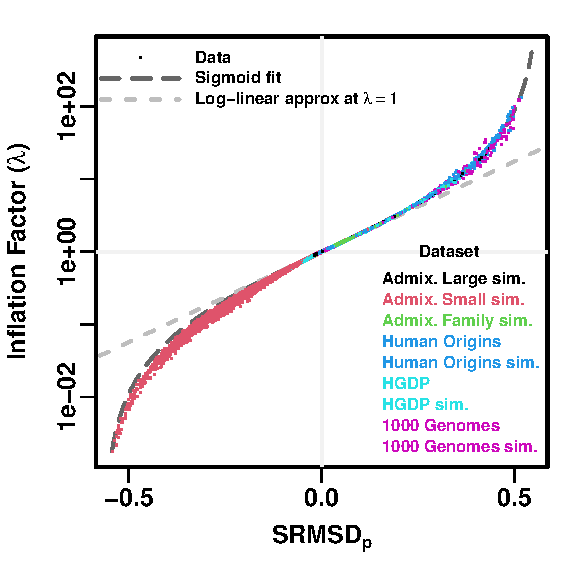
\includegraphics{sum-rmsd-vs-lambda.pdf}
  \caption{
    {\bf Comparison between $\rmsd$ and inflation factor.}
    Each point is a pair of statistics for one replicate, one association model (PCA or LMM with some number of PCs $r$), one trait model (FES vs RC), and one dataset (color coded by dataset).
    Note y-axis ($\lambda$) is on a log scale.
    The sigmoidal curve in \cref{eq:rmsd_lambda_sigmoidal} is fit to the data.
  }
  \label{fig:rmsd_lambda}
\end{figure}

\begin{figure}[hp!]
  \centering
  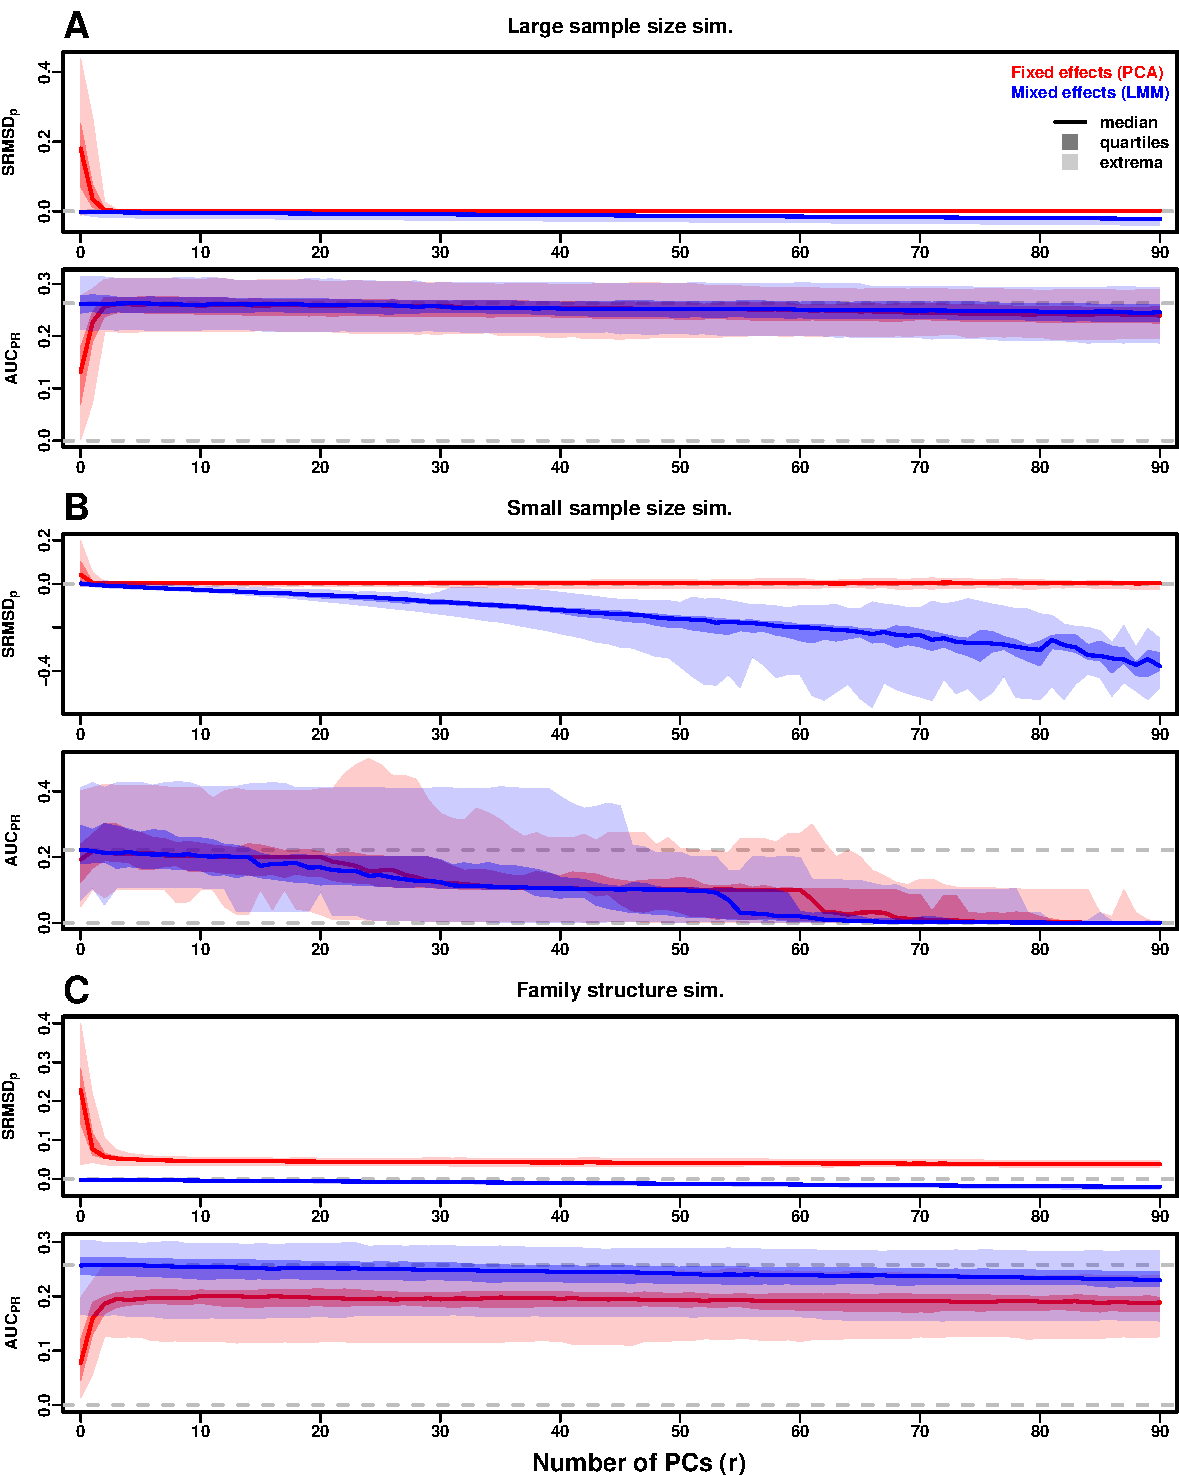
\includegraphics[width=\textwidth,height=\textheight,keepaspectratio]{rmsd-auc-sim.pdf}
  \caption{
    {\small 
      {\bf Evaluations in admixture simulations.}
      Traits simulated from RC model, otherwise the same as \cref{fig:rmsd-auc-sim}.
    }
  }
  \label{fig:rmsd-auc-sim-rc}
\end{figure}

\begin{figure}[hp!]
  \centering
  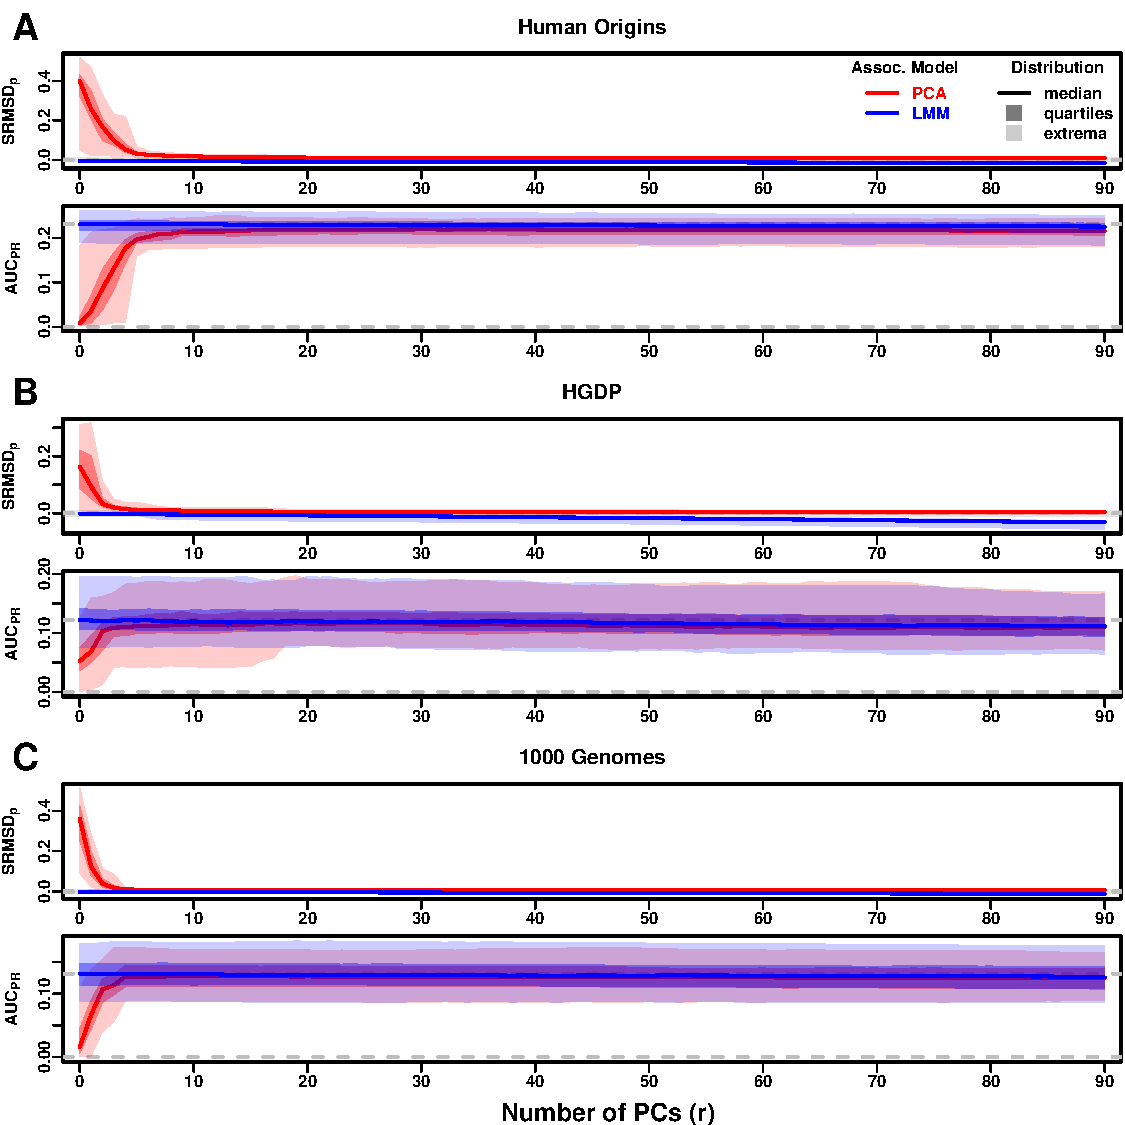
\includegraphics[width=\textwidth,height=\textheight,keepaspectratio]{rmsd-auc-real.pdf}
  \caption{
    {\small 
      {\bf Evaluations in real human genotype datasets.}
      Traits simulated from RC model, otherwise the same as \cref{fig:rmsd-auc-real}.
    }
  }
  \label{fig:rmsd-auc-real-rc}
\end{figure}

\begin{figure}[hp!]
  \centering
  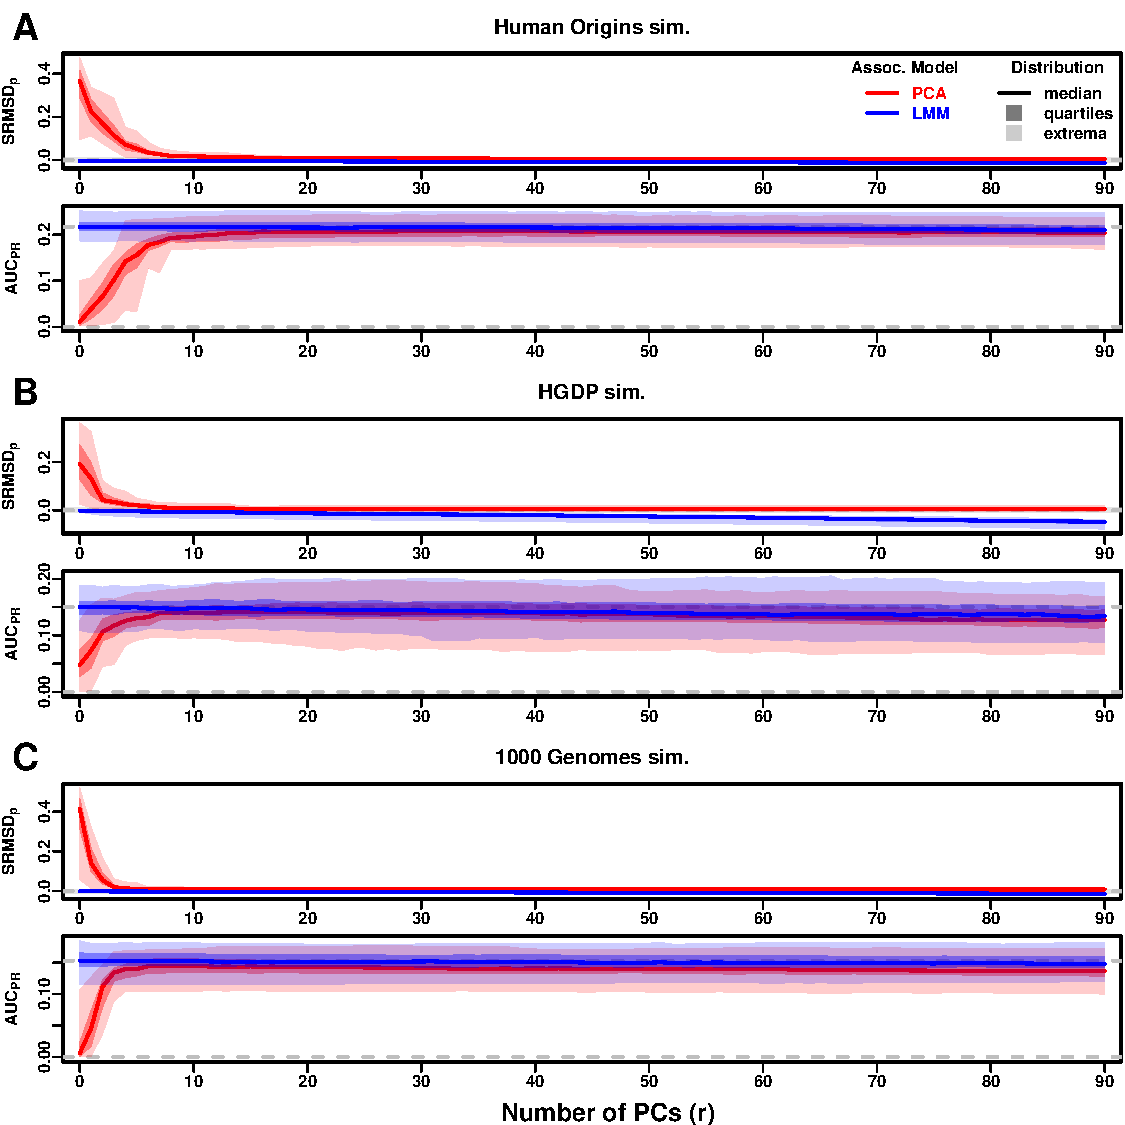
\includegraphics[width=\textwidth,height=\textheight,keepaspectratio]{rmsd-auc-real-sim.pdf}
  \caption{
    {\small 
      {\bf Evaluations in tree simulations fit to human data.}
      Traits simulated from RC model, otherwise the same as \cref{fig:rmsd-auc-real-sim}.
    }
  }
  \label{fig:rmsd-auc-real-sim-rc}
\end{figure}

\begin{figure}[hp!]
  \centering
  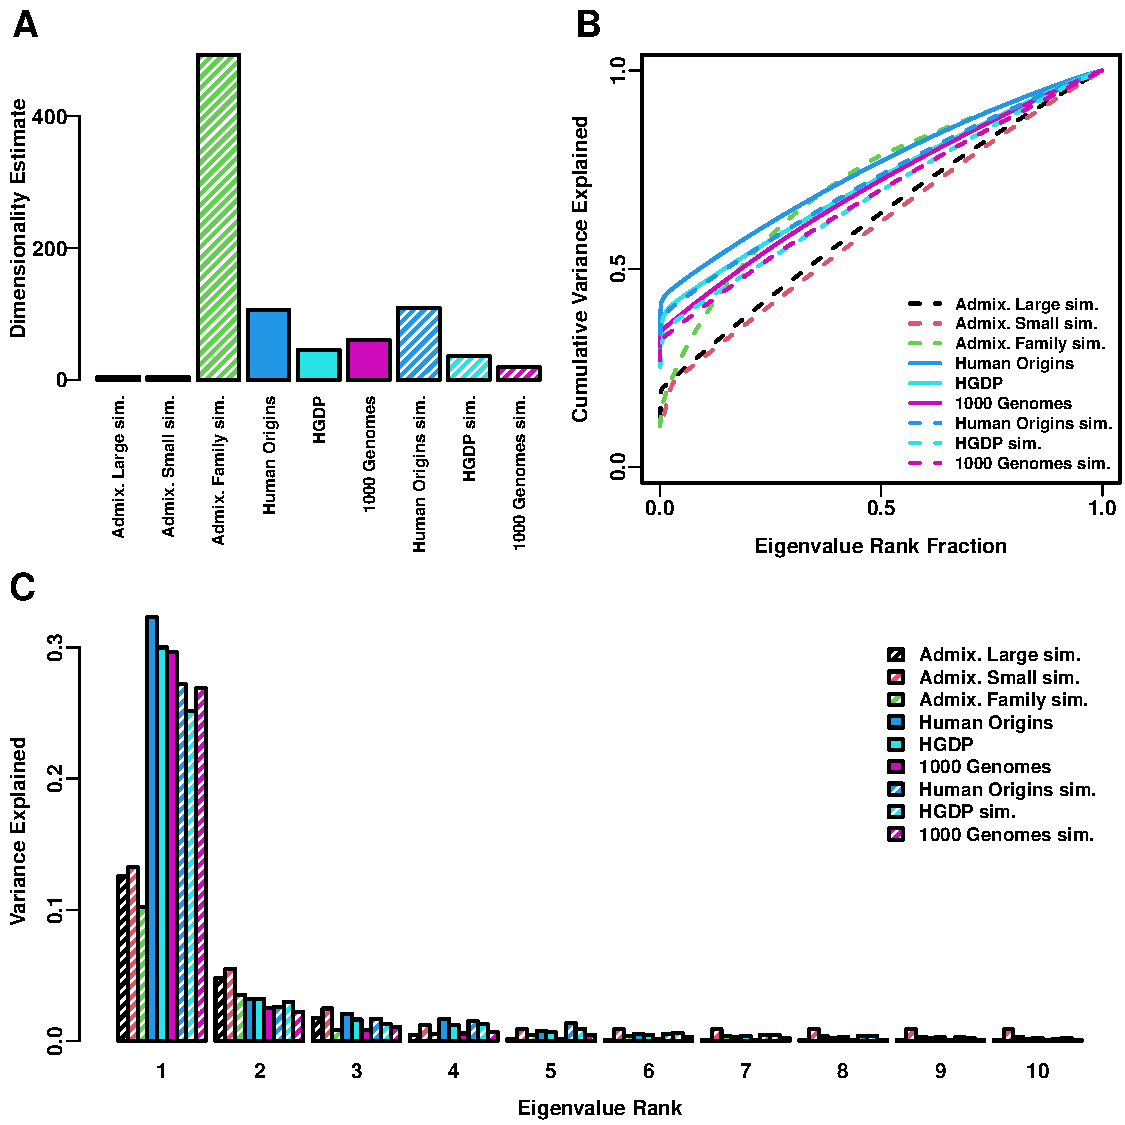
\includegraphics[width=\textwidth]{eigen.pdf}
  \caption{
    {\bf Estimated dimensionality of datasets.}
    \textbf{A.}
    Kinship matrix ranks estimated with the Tracy-Widom test with $p < 0.01$.
    \textbf{B.}
    Cumulative variance explained versus eigenvalue rank fraction.
    \textbf{C.}
    Variance explained by first 10 eigenvalues.
  }
  \label{fig:eigen}
\end{figure}

\clearpage

\section{Supplementary tables}

\begin{table}[hb!]
  \centering
  \footnotesize
  \caption{
    \textbf{Dataset sizes after 4th degree relative filter.}
  }
  \label{tab:king_cutoff}
  % read and automatically format data from a TSV file!
  \sisetup{ table-format = 2, table-number-alignment = right }
  \csvreader[
  tabular = {lSSS},
  separator = tab,
  table head = \toprule Dataset & {Loci ($m$)} & {Ind.~($n$)} & {Ind. removed (\%)} \\\midrule,
  late after last line = \\\bottomrule
  ]{../data/dimensions_king-cutoff-4.txt}{}{\csvlinetotablerow}
\end{table}


\end{document}